%%%%%%%%%%%%%%%%%%%%%%%%%%%%%%%%%%%%%%%%%
%  My documentation report
%  Objetive: Explain what I did and how, so someone can continue with the investigation
%
% Important note:
% Chapter heading images should have a 2:1 width:height ratio,
% e.g. 920px width and 460px height.
%
%%%%%%%%%%%%%%%%%%%%%%%%%%%%%%%%%%%%%%%%%

%----------------------------------------------------------------------------------------
%	PACKAGES AND OTHER DOCUMENT CONFIGURATIONS
%----------------------------------------------------------------------------------------

\documentclass[a4paper,11pt,fleqn]{book} % Default font size and left-justified equations

\usepackage[top=3cm,bottom=3cm,left=3.2cm,right=3.2cm,headsep=10pt,letterpaper]{geometry} % Page margins

\usepackage{xcolor} % Required for specifying colors by name
\definecolor{ocre}{RGB}{52,177,201} % Define the orange color used for highlighting throughout the book

\usepackage[final]{pdfpages} 

% Font Settings
\usepackage{avant} % Use the Avantgarde font for headings
%\usepackage{times} % Use the Times font for headings
\usepackage{mathptmx} % Use the Adobe Times Roman as the default text font together with math symbols from the Sym­bol, Chancery and Com­puter Modern fonts

\usepackage{microtype} % Slightly tweak font spacing for aesthetics
\usepackage[utf8]{inputenc} % Required for including letters with accents
\usepackage[T1]{fontenc} % Use 8-bit encoding that has 256 glyphs

% Bibliography
\usepackage[style=alphabetic,sorting=nyt,sortcites=true,autopunct=true,babel=hyphen,hyperref=true,abbreviate=false,backref=true,backend=biber]{biblatex}
\addbibresource{bibliography.bib} % BibTeX bibliography file
\defbibheading{bibempty}{}

%----------------------------------------------------------------------------------------
%	VARIOUS REQUIRED PACKAGES
%----------------------------------------------------------------------------------------

\usepackage{titlesec} % Allows customization of titles

\usepackage{graphicx} % Required for including pictures
\graphicspath{{Pictures/}} % Specifies the directory where pictures are stored

\usepackage{lipsum} % Inserts dummy text

\usepackage{tikz} % Required for drawing custom shapes

\usepackage[english]{babel} % English language/hyphenation

\usepackage{enumitem} % Customize lists
\setlist{nolistsep} % Reduce spacing between bullet points and numbered lists

\usepackage{booktabs} % Required for nicer horizontal rules in tables

\usepackage{eso-pic} % Required for specifying an image background in the title page

%----------------------------------------------------------------------------------------
%	MAIN TABLE OF CONTENTS
%----------------------------------------------------------------------------------------

\usepackage{titletoc} % Required for manipulating the table of contents

\contentsmargin{0cm} % Removes the default margin
% Chapter text styling
\titlecontents{chapter}[1.25cm] % Indentation
{\addvspace{15pt}\large\sffamily\bfseries} % Spacing and font options for chapters
{\color{ocre!60}\contentslabel[\Large\thecontentslabel]{1.25cm}\color{ocre}} % Chapter number
{}  
{\color{ocre!60}\normalsize\sffamily\bfseries\;\titlerule*[.5pc]{.}\;\thecontentspage} % Page number
% Section text styling
\titlecontents{section}[1.25cm] % Indentation
{\addvspace{5pt}\sffamily\bfseries} % Spacing and font options for sections
{\contentslabel[\thecontentslabel]{1.25cm}} % Section number
{}
{\sffamily\hfill\color{black}\thecontentspage} % Page number
[]
% Subsection text styling
\titlecontents{subsection}[1.25cm] % Indentation
{\addvspace{1pt}\sffamily\small} % Spacing and font options for subsections
{\contentslabel[\thecontentslabel]{1.25cm}} % Subsection number
{}
{\sffamily\;\titlerule*[.5pc]{.}\;\thecontentspage} % Page number
[] 

%----------------------------------------------------------------------------------------
%	MINI TABLE OF CONTENTS IN CHAPTER HEADS
%----------------------------------------------------------------------------------------

% Section text styling
\titlecontents{lsection}[0em] % Indendating
{\footnotesize\sffamily} % Font settings
{}
{}
{}

% Subsection text styling
\titlecontents{lsubsection}[.5em] % Indentation
{\normalfont\footnotesize\sffamily} % Font settings
{}
{}
{}
 
%----------------------------------------------------------------------------------------
%	PAGE HEADERS
%----------------------------------------------------------------------------------------

\usepackage{fancyhdr} % Required for header and footer configuration

\pagestyle{fancy}
\renewcommand{\chaptermark}[1]{\markboth{\sffamily\normalsize\bfseries\chaptername\ \thechapter.\ #1}{}} % Chapter text font settings
\renewcommand{\sectionmark}[1]{\markright{\sffamily\normalsize\thesection\hspace{5pt}#1}{}} % Section text font settings
\fancyhf{} \fancyhead[LE,RO]{\sffamily\normalsize\thepage} % Font setting for the page number in the header
\fancyhead[LO]{\rightmark} % Print the nearest section name on the left side of odd pages
\fancyhead[RE]{\leftmark} % Print the current chapter name on the right side of even pages
\renewcommand{\headrulewidth}{0.5pt} % Width of the rule under the header
\addtolength{\headheight}{2.5pt} % Increase the spacing around the header slightly
\renewcommand{\footrulewidth}{0pt} % Removes the rule in the footer
\fancypagestyle{plain}{\fancyhead{}\renewcommand{\headrulewidth}{0pt}} % Style for when a plain pagestyle is specified

% Removes the header from odd empty pages at the end of chapters
\makeatletter
\renewcommand{\cleardoublepage}{
\clearpage\ifodd\c@page\else
\hbox{}
\vspace*{\fill}
\thispagestyle{empty}
\newpage
\fi}

%----------------------------------------------------------------------------------------
%	THEOREM STYLES
%----------------------------------------------------------------------------------------

\usepackage{amsmath,amsfonts,amssymb,amsthm} % For math equations, theorems, symbols, etc

\newcommand{\intoo}[2]{\mathopen{]}#1\,;#2\mathclose{[}}
\newcommand{\ud}{\mathop{\mathrm{{}d}}\mathopen{}}
\newcommand{\intff}[2]{\mathopen{[}#1\,;#2\mathclose{]}}
\newtheorem{notation}{Notation}[chapter]

%%%%%%%%%%%%%%%%%%%%%%%%%%%%%%%%%%%%%%%%%%%%%%%%%%%%%%%%%%%%%%%%%%%%%%%%%%%
%%%%%%%%%%%%%%%%%%%% dedicated to boxed/framed environements %%%%%%%%%%%%%%
%%%%%%%%%%%%%%%%%%%%%%%%%%%%%%%%%%%%%%%%%%%%%%%%%%%%%%%%%%%%%%%%%%%%%%%%%%%
\newtheoremstyle{ocrenumbox}% % Theorem style name
{0pt}% Space above
{0pt}% Space below
{\normalfont}% % Body font
{}% Indent amount
{\small\bf\sffamily\color{ocre}}% % Theorem head font
{\;}% Punctuation after theorem head
{0.25em}% Space after theorem head
{\small\sffamily\color{ocre}\thmname{#1}\nobreakspace\thmnumber{\@ifnotempty{#1}{}\@upn{#2}}% Theorem text (e.g. Theorem 2.1)
\thmnote{\nobreakspace\the\thm@notefont\sffamily\bfseries\color{black}---\nobreakspace#3.}} % Optional theorem note
\renewcommand{\qedsymbol}{$\blacksquare$}% Optional qed square

\newtheoremstyle{blacknumex}% Theorem style name
{5pt}% Space above
{5pt}% Space below
{\normalfont}% Body font
{} % Indent amount
{\small\bf\sffamily}% Theorem head font
{\;}% Punctuation after theorem head
{0.25em}% Space after theorem head
{\small\sffamily{\tiny\ensuremath{\blacksquare}}\nobreakspace\thmname{#1}\nobreakspace\thmnumber{\@ifnotempty{#1}{}\@upn{#2}}% Theorem text (e.g. Theorem 2.1)
\thmnote{\nobreakspace\the\thm@notefont\sffamily\bfseries---\nobreakspace#3.}}% Optional theorem note

\newtheoremstyle{blacknumbox} % Theorem style name
{0pt}% Space above
{0pt}% Space below
{\normalfont}% Body font
{}% Indent amount
{\small\bf\sffamily}% Theorem head font
{\;}% Punctuation after theorem head
{0.25em}% Space after theorem head
{\small\sffamily\thmname{#1}\nobreakspace\thmnumber{\@ifnotempty{#1}{}\@upn{#2}}% Theorem text (e.g. Theorem 2.1)
\thmnote{\nobreakspace\the\thm@notefont\sffamily\bfseries---\nobreakspace#3.}}% Optional theorem note

%%%%%%%%%%%%%%%%%%%%%%%%%%%%%%%%%%%%%%%%%%%%%%%%%%%%%%%%%%%%%%%%%%%%%%%%%%%
%%%%%%%%%%%%% dedicated to non-boxed/non-framed environements %%%%%%%%%%%%%
%%%%%%%%%%%%%%%%%%%%%%%%%%%%%%%%%%%%%%%%%%%%%%%%%%%%%%%%%%%%%%%%%%%%%%%%%%%
\newtheoremstyle{ocrenum}% % Theorem style name
{5pt}% Space above
{5pt}% Space below
{\normalfont}% % Body font
{}% Indent amount
{\small\bf\sffamily\color{ocre}}% % Theorem head font
{\;}% Punctuation after theorem head
{0.25em}% Space after theorem head
{\small\sffamily\color{ocre}\thmname{#1}\nobreakspace\thmnumber{\@ifnotempty{#1}{}\@upn{#2}}% Theorem text (e.g. Theorem 2.1)
\thmnote{\nobreakspace\the\thm@notefont\sffamily\bfseries\color{black}---\nobreakspace#3.}} % Optional theorem note
\renewcommand{\qedsymbol}{$\blacksquare$}% Optional qed square
\makeatother

% Defines the theorem text style for each type of theorem to one of the three styles above
\newcounter{dummy} 
\numberwithin{dummy}{section}
\theoremstyle{ocrenumbox}
\newtheorem{theoremeT}[dummy]{Theorem}
\newtheorem{problem}{Problem}[chapter]
\newtheorem{exerciseT}{Exercise}[chapter]
\theoremstyle{blacknumex}
\newtheorem{exampleT}{Example}[chapter]
\theoremstyle{blacknumbox}
\newtheorem{vocabulary}{Vocabulary}[chapter]
\newtheorem{definitionT}{Definition}[section]
\newtheorem{corollaryT}[dummy]{Corollary}
\theoremstyle{ocrenum}
\newtheorem{proposition}[dummy]{Proposition}

%----------------------------------------------------------------------------------------
%	DEFINITION OF COLORED BOXES
%----------------------------------------------------------------------------------------

\RequirePackage[framemethod=default]{mdframed} % Required for creating the theorem, definition, exercise and corollary boxes

% Theorem box
\newmdenv[skipabove=7pt,
skipbelow=7pt,
backgroundcolor=black!5,
linecolor=ocre,
innerleftmargin=5pt,
innerrightmargin=5pt,
innertopmargin=5pt,
leftmargin=0cm,
rightmargin=0cm,
innerbottommargin=5pt]{tBox}

% Exercise box	  
\newmdenv[skipabove=7pt,
skipbelow=7pt,
rightline=false,
leftline=true,
topline=false,
bottomline=false,
backgroundcolor=ocre!10,
linecolor=ocre,
innerleftmargin=5pt,
innerrightmargin=5pt,
innertopmargin=5pt,
innerbottommargin=5pt,
leftmargin=0cm,
rightmargin=0cm,
linewidth=4pt]{eBox}	

% Definition box
\newmdenv[skipabove=7pt,
skipbelow=7pt,
rightline=false,
leftline=true,
topline=false,
bottomline=false,
linecolor=ocre,
innerleftmargin=5pt,
innerrightmargin=5pt,
innertopmargin=0pt,
leftmargin=0cm,
rightmargin=0cm,
linewidth=4pt,
innerbottommargin=0pt]{dBox}	

% Corollary box
\newmdenv[skipabove=7pt,
skipbelow=7pt,
rightline=false,
leftline=true,
topline=false,
bottomline=false,
linecolor=gray,
backgroundcolor=black!5,
innerleftmargin=5pt,
innerrightmargin=5pt,
innertopmargin=5pt,
leftmargin=0cm,
rightmargin=0cm,
linewidth=4pt,
innerbottommargin=5pt]{cBox}

% Creates an environment for each type of theorem and assigns it a theorem text style from the "Theorem Styles" section above and a colored box from above
\newenvironment{theorem}{\begin{tBox}\begin{theoremeT}}{\end{theoremeT}\end{tBox}}
\newenvironment{exercise}{\begin{eBox}\begin{exerciseT}}{\hfill{\color{ocre}\tiny\ensuremath{\blacksquare}}\end{exerciseT}\end{eBox}}				  
\newenvironment{definition}{\begin{dBox}\begin{definitionT}}{\end{definitionT}\end{dBox}}	
\newenvironment{example}{\begin{exampleT}}{\hfill{\tiny\ensuremath{\blacksquare}}\end{exampleT}}		
\newenvironment{corollary}{\begin{cBox}\begin{corollaryT}}{\end{corollaryT}\end{cBox}}	

%----------------------------------------------------------------------------------------
%	REMARK ENVIRONMENT
%----------------------------------------------------------------------------------------

\newenvironment{remark}{\par\vspace{10pt}\small % Vertical white space above the remark and smaller font size
\begin{list}{}{
\leftmargin=35pt % Indentation on the left
\rightmargin=25pt}\item\ignorespaces % Indentation on the right
\makebox[-2.5pt]{\begin{tikzpicture}[overlay]
\node[draw=ocre!60,line width=1pt,circle,fill=ocre!25,font=\sffamily\bfseries,inner sep=2pt,outer sep=0pt] at (-15pt,0pt){\textcolor{ocre}{R}};\end{tikzpicture}} % Orange R in a circle
\advance\baselineskip -1pt}{\end{list}\vskip5pt} % Tighter line spacing and white space after remark

%----------------------------------------------------------------------------------------
%	SECTION NUMBERING IN THE MARGIN
%----------------------------------------------------------------------------------------

\makeatletter
\renewcommand{\@seccntformat}[1]{\llap{\textcolor{ocre}{\csname the#1\endcsname}\hspace{1em}}}                    
\renewcommand{\section}{\@startsection{section}{1}{\z@}
{-4ex \@plus -1ex \@minus -.4ex}
{1ex \@plus.2ex }
{\normalfont\large\sffamily\bfseries}}
\renewcommand{\subsection}{\@startsection {subsection}{2}{\z@}
{-3ex \@plus -0.1ex \@minus -.4ex}
{0.5ex \@plus.2ex }
{\normalfont\sffamily\bfseries}}
\renewcommand{\subsubsection}{\@startsection {subsubsection}{3}{\z@}
{-2ex \@plus -0.1ex \@minus -.2ex}
{.2ex \@plus.2ex }
{\normalfont\small\sffamily\bfseries}}                        
\renewcommand\paragraph{\@startsection{paragraph}{4}{\z@}
{-2ex \@plus-.2ex \@minus .2ex}
{.1ex}
{\normalfont\small\sffamily\bfseries}}

%----------------------------------------------------------------------------------------
%	HYPERLINKS IN THE DOCUMENTS
%----------------------------------------------------------------------------------------

% For an unclear reason, the package should be loaded now and not later
\usepackage{hyperref}
\hypersetup{hidelinks,backref=true,pagebackref=true,hyperindex=true,colorlinks=false,breaklinks=true,urlcolor= ocre,bookmarks=true,bookmarksopen=false,pdftitle={Title},pdfauthor={Author}}

%----------------------------------------------------------------------------------------
%	CHAPTER HEADINGS
%----------------------------------------------------------------------------------------

% The set-up below should be (sadly) manually adapted to the overall margin page septup controlled by the geometry package loaded in the main.tex document. It is possible to implement below the dimensions used in the goemetry package (top,bottom,left,right)... TO BE DONE

\newcommand{\thechapterimage}{}
\newcommand{\chapterimage}[1]{\renewcommand{\thechapterimage}{#1}}

% Numbered chapters with mini tableofcontents
\def\thechapter{\arabic{chapter}}
\def\@makechapterhead#1{
\thispagestyle{empty}
{\centering \normalfont\sffamily
\ifnum \c@secnumdepth >\m@ne
\if@mainmatter
\startcontents
\begin{tikzpicture}[remember picture,overlay]
\node at (current page.north west)
{\begin{tikzpicture}[remember picture,overlay]
\node[anchor=north west,inner sep=0pt] at (0,0) {\includegraphics[width=\paperwidth]{\thechapterimage}};
%%%%%%%%%%%%%%%%%%%%%%%%%%%%%%%%%%%%%%%%%%%%%%%%%%%%%%%%%%%%%%%%%%%%%%%%%%%%%%%%%%%%%
% Commenting the 3 lines below removes the small contents box in the chapter heading
%\fill[color=ocre!10!white,opacity=.6] (1cm,0) rectangle (8cm,-7cm);
%\node[anchor=north west] at (1.1cm,.35cm) {\parbox[t][8cm][t]{6.5cm}{\huge\bfseries\flushleft \printcontents{l}{1}{\setcounter{tocdepth}{2}}}};
\draw[anchor=west] (5cm,-9cm) node [rounded corners=20pt,fill=ocre!10!white,text opacity=1,draw=ocre,draw opacity=1,line width=1.5pt,fill opacity=.6,inner sep=12pt]{\huge\sffamily\bfseries\textcolor{black}{\thechapter. #1\strut\makebox[22cm]{}}};
%%%%%%%%%%%%%%%%%%%%%%%%%%%%%%%%%%%%%%%%%%%%%%%%%%%%%%%%%%%%%%%%%%%%%%%%%%%%%%%%%%%%%
\end{tikzpicture}};
\end{tikzpicture}}
\par\vspace*{230\p@}
\fi
\fi}

% Unnumbered chapters without mini tableofcontents (could be added though) 
\def\@makeschapterhead#1{
\thispagestyle{empty}
{\centering \normalfont\sffamily
\ifnum \c@secnumdepth >\m@ne
\if@mainmatter
\begin{tikzpicture}[remember picture,overlay]
\node at (current page.north west)
{\begin{tikzpicture}[remember picture,overlay]
\node[anchor=north west,inner sep=0pt] at (0,0) {\includegraphics[width=\paperwidth]{\thechapterimage}};
\draw[anchor=west] (5cm,-9cm) node [rounded corners=20pt,fill=ocre!10!white,fill opacity=.6,inner sep=12pt,text opacity=1,draw=ocre,draw opacity=1,line width=1.5pt]{\huge\sffamily\bfseries\textcolor{black}{#1\strut\makebox[22cm]{}}};
\end{tikzpicture}};
\end{tikzpicture}}
\par\vspace*{230\p@}
\fi
\fi
}
\makeatother % Insert the commands.tex file which contains the majority of the structure behind the template

\begin{document}
%----------------------------------------------------------------------------------------
%	TITLE PAGE
%----------------------------------------------------------------------------------------

\begingroup
\thispagestyle{empty}
\AddToShipoutPicture*{\put(0,0){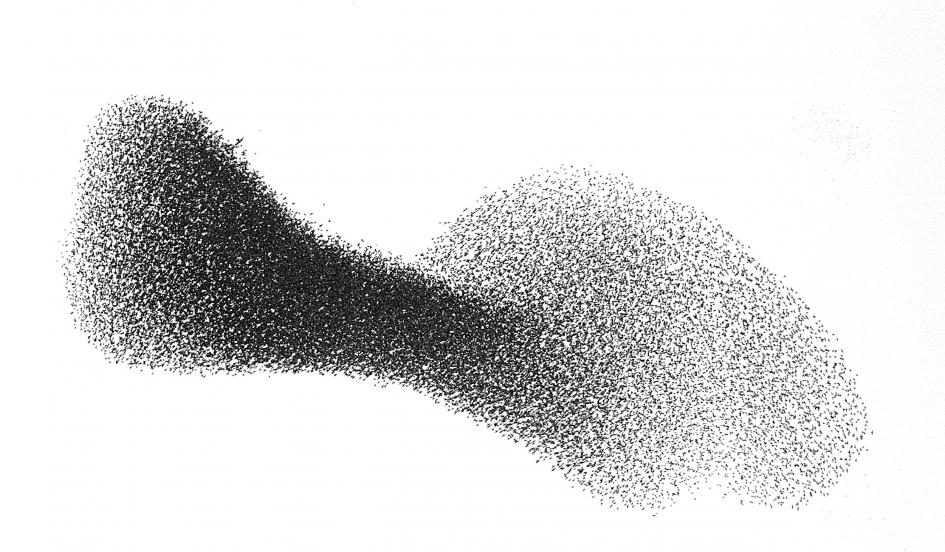
\includegraphics[scale=0.68]{swarm}}} % Image background
\centering
\vspace*{5cm}
\par\normalfont\fontsize{35}{35}\sffamily\selectfont
\textcolor{black}{Dossier de demande \\de qualification \\aux fonctions de \\Maître de Conférences}\\
\textcolor{black}{\LARGE Section 67 - Groupe X}\par % Book title
\vspace*{1cm}
\textcolor{black}{\Huge Julien Boulay}\par % Author name
\endgroup

\clearpage

\begin{flushright}
Dossier à l'attention de Mme Christine \textsc{Pergent-Martini}\\ 355 route di u Lagu\\ 20290 LUCCIANA
\end{flushright}
%----------------------------------------------------------------------------------------
%	TABLE OF CONTENTS
%----------------------------------------------------------------------------------------

 % Table of contents heading image

\pagestyle{empty} % No headers

\chapterimage{blank}

\tableofcontents % Print the table of contents itself

%\cleardoublepage % Forces the first chapter to start on an odd page so it's on the right

\pagestyle{fancy} % Print headers again


%----------------------------------------------------------------------------------------
%	CHAPTER 1
%----------------------------------------------------------------------------------------
\chapterimage{blank}
\chapter{Curriculum Vitae - 2 pages}
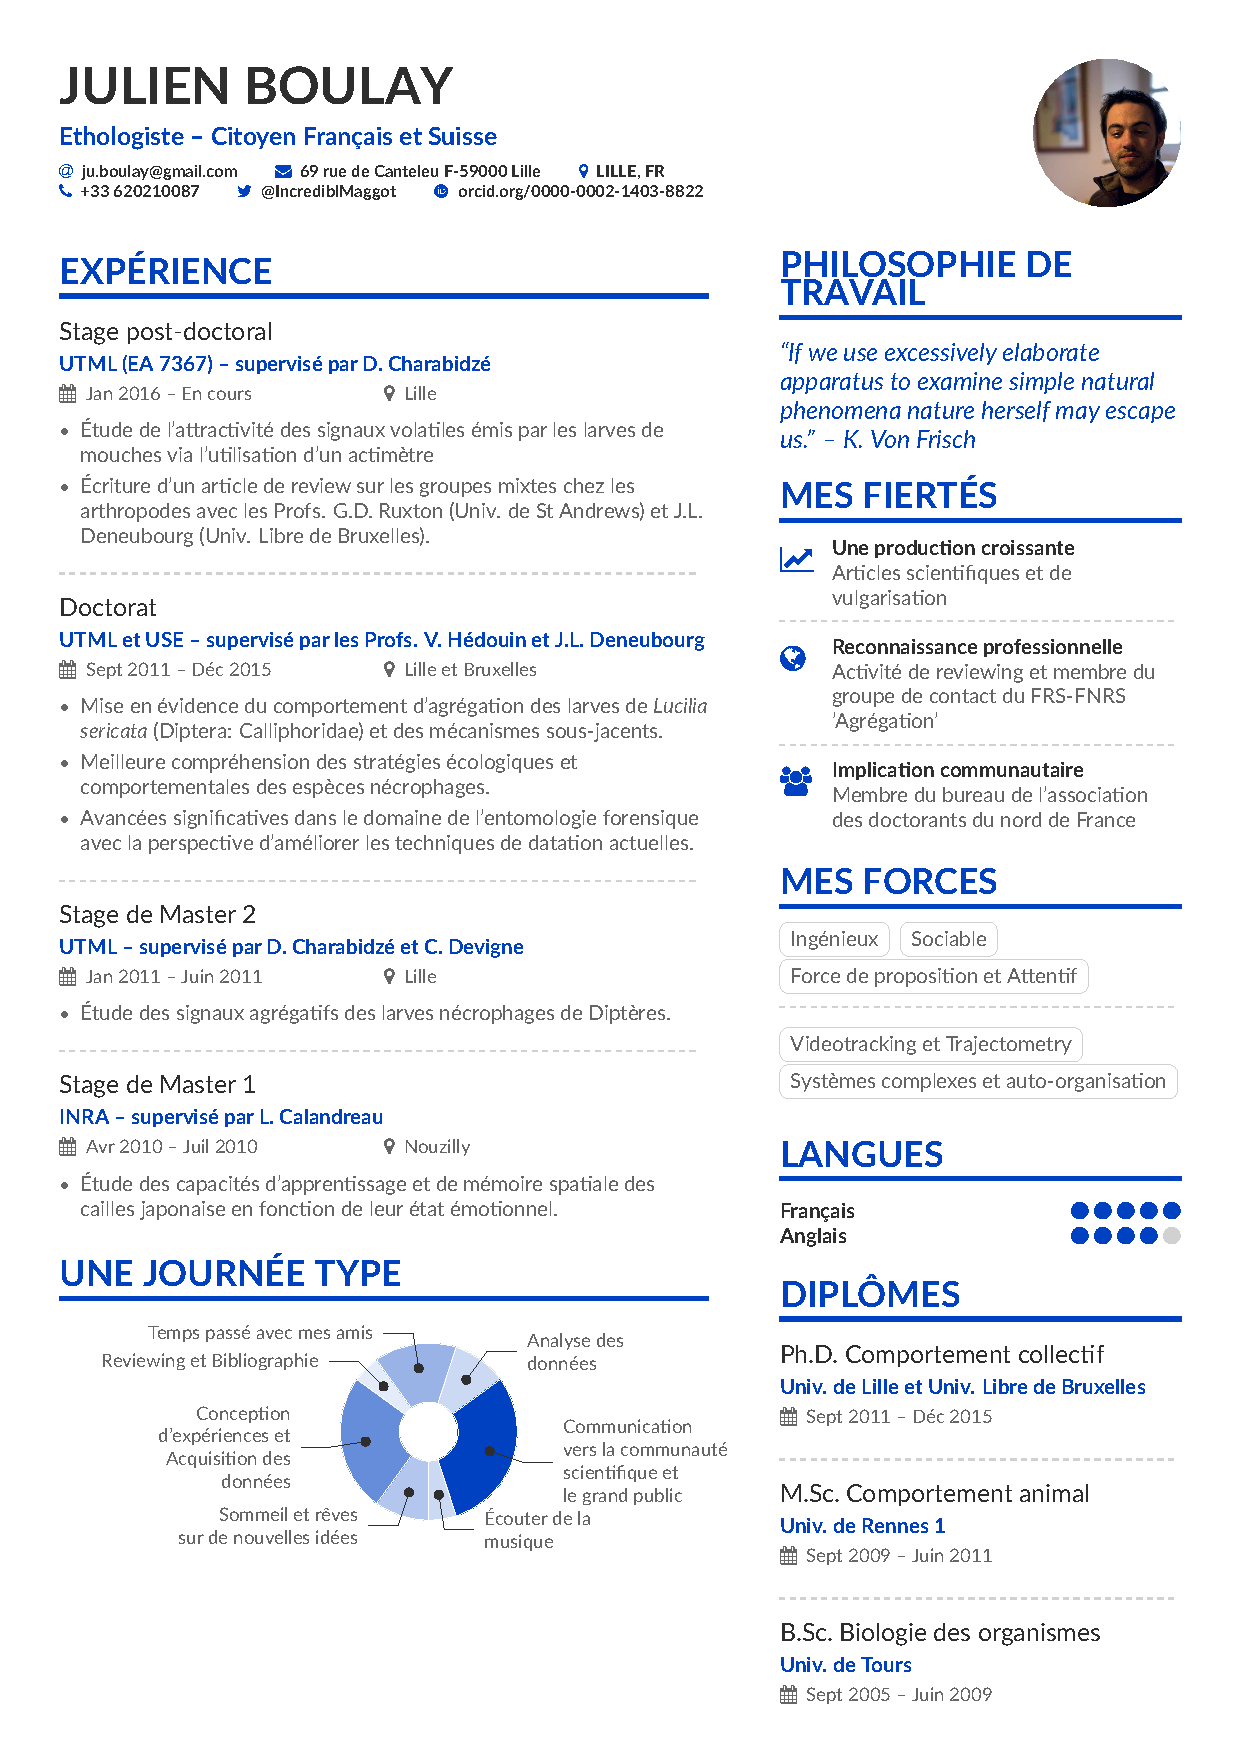
\includepdf[pages=1-2]{cv-french.pdf}

%----------------------------------------------------------------------------------------
%	CHAPTER 2
%----------------------------------------------------------------------------------------
\chapterimage{blank}

\chapter{Rapport d'activités - 4 pages}
\clearpage

\section{Activités de recherche}\index{Activités de recherche}
\subsection{Contexte}
Les comportements collectifs sont observés dans tous les taxons animaux allant des micro-organismes aux humains. Chez certaines espèces sociales, comme les étourneaux ou les criquets, ces regroupements peuvent rassembler des milliers d’individus formant d’impressionnantes structures collectives. Ces groupes sont régit par des règles comportementales (e.g. interactions interindividuelles) qui répétées de nombreuses fois aboutissent à la formation de systèmes auto-organisés complexes (i.e. théorie de l’auto-organisation). La compréhension des facteurs clés qui permettent l’émergence des décisions collectives prises par de larges groupes est fondamentale pour déchiffrer l’évolution de la socialité. L’étude des comportements collectifs est essentiellement basée sur des situations monospécifiques (une seule espèce formant un groupe social). Ces travaux se sont focalisés généralement sur les mécanismes qui gouvernent l’évolution et le maintien de ces groupes chez différentes espèces. Mieux comprendre ces phénomènes implique dès lors l’étude des différents comportements et moyens de communication qui interviennent dans la formation des groupes et la coopération entre individus. C’est dans ce contexte fondamental que mes recherches (doctorales et post-doctorales) s’inscrivent.

\subsection{Objectifs et approches}
Mes recherches actuelles, et que j’aimerai poursuivre, s’intéressent à comprendre les mécanismes qui sous-tendent les regroupement d’individus. Je m’attache à étudier comment les structures collectives émergentes se forment, se maintiennent et se régulent dans le temps. J'étudie également les choix que ces groupes sont capables de faire. La prise de décision collective, \textit{collective decision-making}, joue un rôle central dans la vie des animaux sociaux. Pour étudier cela, je privilégie une approche comportementale couplée à des phases de modélisation.

En parallèle, je m’intéresse aux phénomènes de coopération-compétition observés dans des groupes hétérospécifique (plus d’une espèce dans un même groupe social) et plus spécialement chez les arthropodes. Ces groupes nous offrent un angle d'étude particulièrement intéressant sur ces phénomènes et notamment sur le processus de spéciation sympatrique.

Ces différents sujets je les ai abordé au cours de ma thèse (2011-15) effectuée en cotutelle entre l'Unité de Taphonomie Médico-Légale (UTML - EA 7367) de l'Université de Lille sous la direction du Prof. Valéry \textsc{Hédouin} (PU-PH) et de Damien \textsc{Charabidzé} (MCF) et l'Unité d'Écologie Sociale (USE) de l'Université Libre de Bruxelles sous la direction du Prof. Jean-Louis \textsc{Deneubourg}. J'ai également pu les poursuivre lors d'une année de contrat post-doctoral effectuée au sein de l'UTML sous la direction de D. \textsc{Charabidzé}.

\subsection{Période doctorale 2011-15 | UTML (EA 7367) et USE}
Le comportement d'agrégation est considéré comme le premier pas vers des niveaux de socialité supérieurs. La compréhension des facteurs clés permettant l’émergence des décisions collectives chez les groupes composés d’individus simples (ayant une connaissance limitée de leur environnement) est donc fondamentale pour étudier l’évolution de la socialité. A l'heure actuelle, la majorité des études se sont focalisées sur les espèces les plus sociales, et notamment celles formant des groupes monospécifiques. \textit{A contrario}, les larves nécrophages de Diptères (asticots) forment sur un même cadavre des agrégats hétérospécifiques pouvant contenir des milliers d'individus, leur offrant divers bénéfices (e.g. production de chaleur, d’enzymes). 

De part ces observations \textit{in natura}, ces insectes apparaissent être un bon modèle biologique dans un contexte évolutif d'étude des comportements collectifs. Mon travail de thèse s'est attaché à mettre en évidence et quantifier les phénomènes d'agrégation des larves de \textit{Lucilia sericata} (Diptera: Calliphoridae) et les mécanismes qui sous-tendent ces regroupements. Après une description introductive des groupes hétérospécifiques chez les arthropodes, j'ai démontré pour la première fois expérimentalement l'existence d'un comportement d’agrégation actif des larves (suivi dans le temps d'un groupe sur un milieu homogène). J'ai également mis en évidence l'effet d'attraction/rétention sur les larves d'un composé cuticulaire déposé au sol par les individus et reconnu par leurs congénères. Cette reconnaissance se fait probablement via l'utilisation d'un comportement exploratoire caractéristique que j'ai décrit, quantifié et nommé: le scanning. J'ai ensuite passé une semaine en formation chez le Prof. Georges \textsc{Lognay} (Gembloux Agro-Bio-Tech) afin d'identifier la composition de ce signal cuticulaire via des techniques de GC-MS.

Puis, j'ai mis en évidence la capacité des larves de deux espèces proches phylogénétiquement et écologiquement, \textit{L. sericata} et \textit{Calliphora vomitoria}, à faire un choix collectif en groupe monospécifique comme en hétérospécifique (choix binaire entre deux sites de nourriture). Ces résultats suggèrent l'existence d'une reconnaissance interspécifique de vecteurs d'agrégation (e.g. le signal larvaire). Enfin, j'ai mis en évidence l'existence de préférendums thermiques chez ces espèces, et la capacité des larves à sélectionner collectivement cette température préférentielle. Ma thèse s'est inscrite dans deux contextes bien distincts : un fondamental qui est l'étude des comportements collectifs et le second, que l'on peut qualifier d'applicatif, qui est l'entomologie forensique. Dans son ensemble, ce travail a offert des connaissances inédites sur la vie de ces groupes. Il ouvre des perspectives d'étude prometteuses sur les comportements collectifs interspécifiques et les bénéfices évolutifs liés à l'agrégation. 


\subsection{Période post-doctorale 2016-. | UTML (EA 7367)}
A l'heure actuelle, je termine mon contrat post-doctoral d'un an au sein de l'UTML. Lors de cette année, j'ai étudié l'éventuelle attraction à distance du composé cuticulaire déposé au sol par les larves nécrophages de Diptères (mis en évidence dans le cadre de ma thèse). Pour cela j'ai étudié l'activité locomotrice des larves nécrophages face à différents signaux olfactifs pertinents (nourriture, congénères) à l'aide d'un actimètre. 
J'ai également utilisé cette année pour écrire une revue exhaustive sur les groupes hétérospécifiques rencontrés chez les arthropodes. Cette compilation d'articles a été écrite au regard du contexte de l'étude des comportements collectifs. Écrite en collaboration avec les Profs. G. D. \textsc{Ruxton} (Université de St Andrews) et J. L. \textsc{Deneubourg} (Université Libre de Bruxelles), elle est actuellement dans les mains des reviewers de la revue \textit{The Quarterly Review of Biology}.

La compréhension des groupes hétérospécifiques et l’utilisation d’une démarche comparative sont deux axes innovants dans le contexte de l’étude des comportements collectifs. Mes études permettront de nous renseigner sur la frontière étroite entre coopération et compétition présente au sein de ces groupes sociaux. D’une manière générale, mes résultats apporteront des données inédites sur la compréhension de tels groupes sociaux dans une démarche évolutionniste de l’étude des sociétés dans le règne animal. De plus, ils permettront d’avoir une vue globale sur les relations/interactions entre plusieurs espèces membres d’un même groupe social. Du côté applicatif, mes recherches permettront de mieux gérer les conditions d’élevages d’espèces proches vivant à proximité les unes des autres.

Lors de cette année de post-doctorat à l'UTML, j'ai également déposé deux bourses post-doctorales (Human Frontier et Fonds National Suisse) pour un séjour au sein du laboratoire de Jérôme \textsc{Buhl} (School of Agriculture, Food and Wine - Université d'Adélaïde, Australie). Le projet déposé est d'étudier la différence de pattern d'agrégation observée chez deux espèces de criquets nuisibles, l'espèce australienne (\textit{Chortoicetes terminifera}) et une espèce sud-africaine (\textit{Locustana pardalina}). Le but est de mettre en évidence les facteurs comportementaux et/ou environnementaux responsables de cette différence de pattern. Lors de ce séjour, je prévois de me familiariser avec les techniques d'observation de masses d'insectes (pilotage de drones) et de renforcer de manière significative mes connaissances en modélisation mathématique des comportements collectifs.


\section{Activités d'enseignement}\index{Activités d'enseignement}

Lors de mes premières années de doctorant (2012-13), j'ai eu l'opportunité d'encadrer des travaux pratiques en Zoologie au sein de l'Université Catholique de Lille (Tableau \ref{tab:enseignement}). Ces heures de TP, dispensées aux étudiant(e)s de Licence Sciences, Technologies, Santé Mention Biologie, étaient essentiellement des dissections d'animaux divers (arthropodes et petits mammifères). En 2013, j'ai dispensé quelques heures de travaux dirigés à des étudiant(e)s de médecine en première année du Master Biologie-Santé Parcours Santé Option Physiologie/Physiopathologie (Tableau \ref{tab:enseignement}). Lors de ces TD, je leur ai introduit les concepts de base de l'éthologie ainsi que des généralités sur l'entomologie (anatomie, physiologie et comportement).

En 2014, j'ai encadré des TP d'identification d'insectes et de datation entomologique du décès à des étudiant(e)s de médecine en première année du Master Biologie-Santé Parcours Santé Option Physiologie/Physiopathologie (Tableau \ref{tab:enseignement}). Ces TP consistaient à identifier trois espèces d'insectes nécrophages à l'aide de clefs dichotomiques. Puis, je demandais aux étudiants d'effectuer une datation entomologique du décès basée sur les durées de développement des insectes à l'aide de la base de données disponible sur le site ForenSeek (\textit{www.forenseek.org}). Ce site est l'aboutissement de la thèse de mon co-directeur de thèse Damien \textsc{Charabidzé}.

Enfin en 2016, j'ai dispensé des travaux dirigés à des médecins se spécialisant en médecine légale en intégrant le DESC (Diplôme Spécialisé d’Études Complémentaires de Médecine légale et expertises médicales). Lors de ces cours, j'ai introduit les notions de base de l'entomologie médico-légale (identification des espèces nécrophages, étude de cas, datation entomologique). 

\begin{table}[h!]
	\caption{Résumé des enseignements. DESC : Diplôme Spécialisé d’Études Complémentaires (Médecine légale). Volume horaire exprimé en équivalent TD.}
	\label{tab:enseignement}
	\centering
	\begin{tabular*}{\linewidth}{@{\extracolsep{\fill}}ccccc}
		 \toprule
         \textbf{Discipline}				& \textbf{Niveau}		& \textbf{Année}		& \textbf{Nature}		& \textbf{Volume horaire}\\
		 \midrule
		Zoologie	&L2		&2012-13		&TP		&36h\\
        Comportement animal	&M1	&2013	&TD	&6h\\
        Identification et datation entomologique	&M1	&2014	&TP	&16h\\
        Entomologie médico-légale	&DESC	&2016	&TD	&12h\\
        \bottomrule
        \end{tabular*}
        \end{table}
        
Lors de mes années de doctorat, j'ai eu le plaisir d'encadrer les stages de recherche d'étudiant(e)s passionné(e)s et passionnant(e)s de tous niveaux (cf. Attestation d'encadrements). Ces jeunes scientifiques étaient pour la plupart des étudiant(e)s se spécialisant en éthologie et en écologie comportementale (Master Comportement Animal et Humain de l'Université de Rennes 1, Master Eco-Etho de l'Université de St Étienne et Master Éthologie de l'Université de Paris XIII). 

\section{Charges collectives}\index{Charges collectives}

Lors de mon doctorat, j'ai attaché une certaine importance à mon implication dans la vie associative. J'ai participé au relancement de l'association BioAddoct (association des Docteurs et Doctorants en Biologie et Santé du Nord de France - \textit{www.bioaddoct.fr}) créée en 2009 et tombée en désuétude après 2011. Les années 2012-13 ont permis à cette association de renaître et ma participation fût pleine lors de l'année 2014 en ma qualité de chargé de communication. Ma contribution consistait à m'occuper de la charte graphique et à la création de supports visuels pour les événements organisés par cette association.

En 2014, j'ai participé à l'organisation du congrès annuel de l'EAFE (European Association for Forensic Entomology - \textit{www.eafe.org}) tenu à Lille. Cette association réunie les scientifiques de toute l'Europe étudiant les insectes nécrophages d'un point de vue fondamental (comportement, physiologie, identification) et appliqué (techniques de datation du décès, expertises).

%----------------------------------------------------------------------------------------
%	CHAPTER 3
%--------------------------------------------------------------------------------------
\chapterimage{blank}

\chapter{Trois publications}

\begin{itemize} 
\item[\tiny{$\blacksquare$}] ARTICLE 1\\
\textsc{\textbf{Boulay J.}}, \textsc{Devigne} C., \textsc{Gosset} D. and \textsc{Charabidzé} D. Evidence of active aggregation behaviour in \textit{Lucilia sericata} larvae and possible implication of a conspecific mark. Article publié dans \emph{Animal Behaviour}, 85:6, 1191-1197, 2013.\\
\end{itemize}

\begin{itemize} 
\item[\tiny{$\blacksquare$}] ARTICLE 2\\
\textbf{\textsc{Boulay} J.}, \textsc{Betremieux} C., \textsc{Hédouin} V. and \textsc{Charabidzé} D. A first insight in the scanning behaviour of presocial blow fly larvae. Article publié dans \emph{Physiological Entomology}, DOI: 10.1111/phen.12117. 2015.\\
\end{itemize}

\begin{itemize} 
\item[\tiny{$\blacksquare$}] ARTICLE 3\\
\textsc{\textbf{Boulay J.}}, \textsc{Deneubourg} J.-L., \textsc{Hédouin} V. and \textsc{Charabidzé} D. Interspecific shared collective decision-making in two forensically important species. Article publié dans \emph{Proceedings of the Royal Society B}, DOI: 10.1098/rspb.2015.2676. 2016.
\end{itemize}


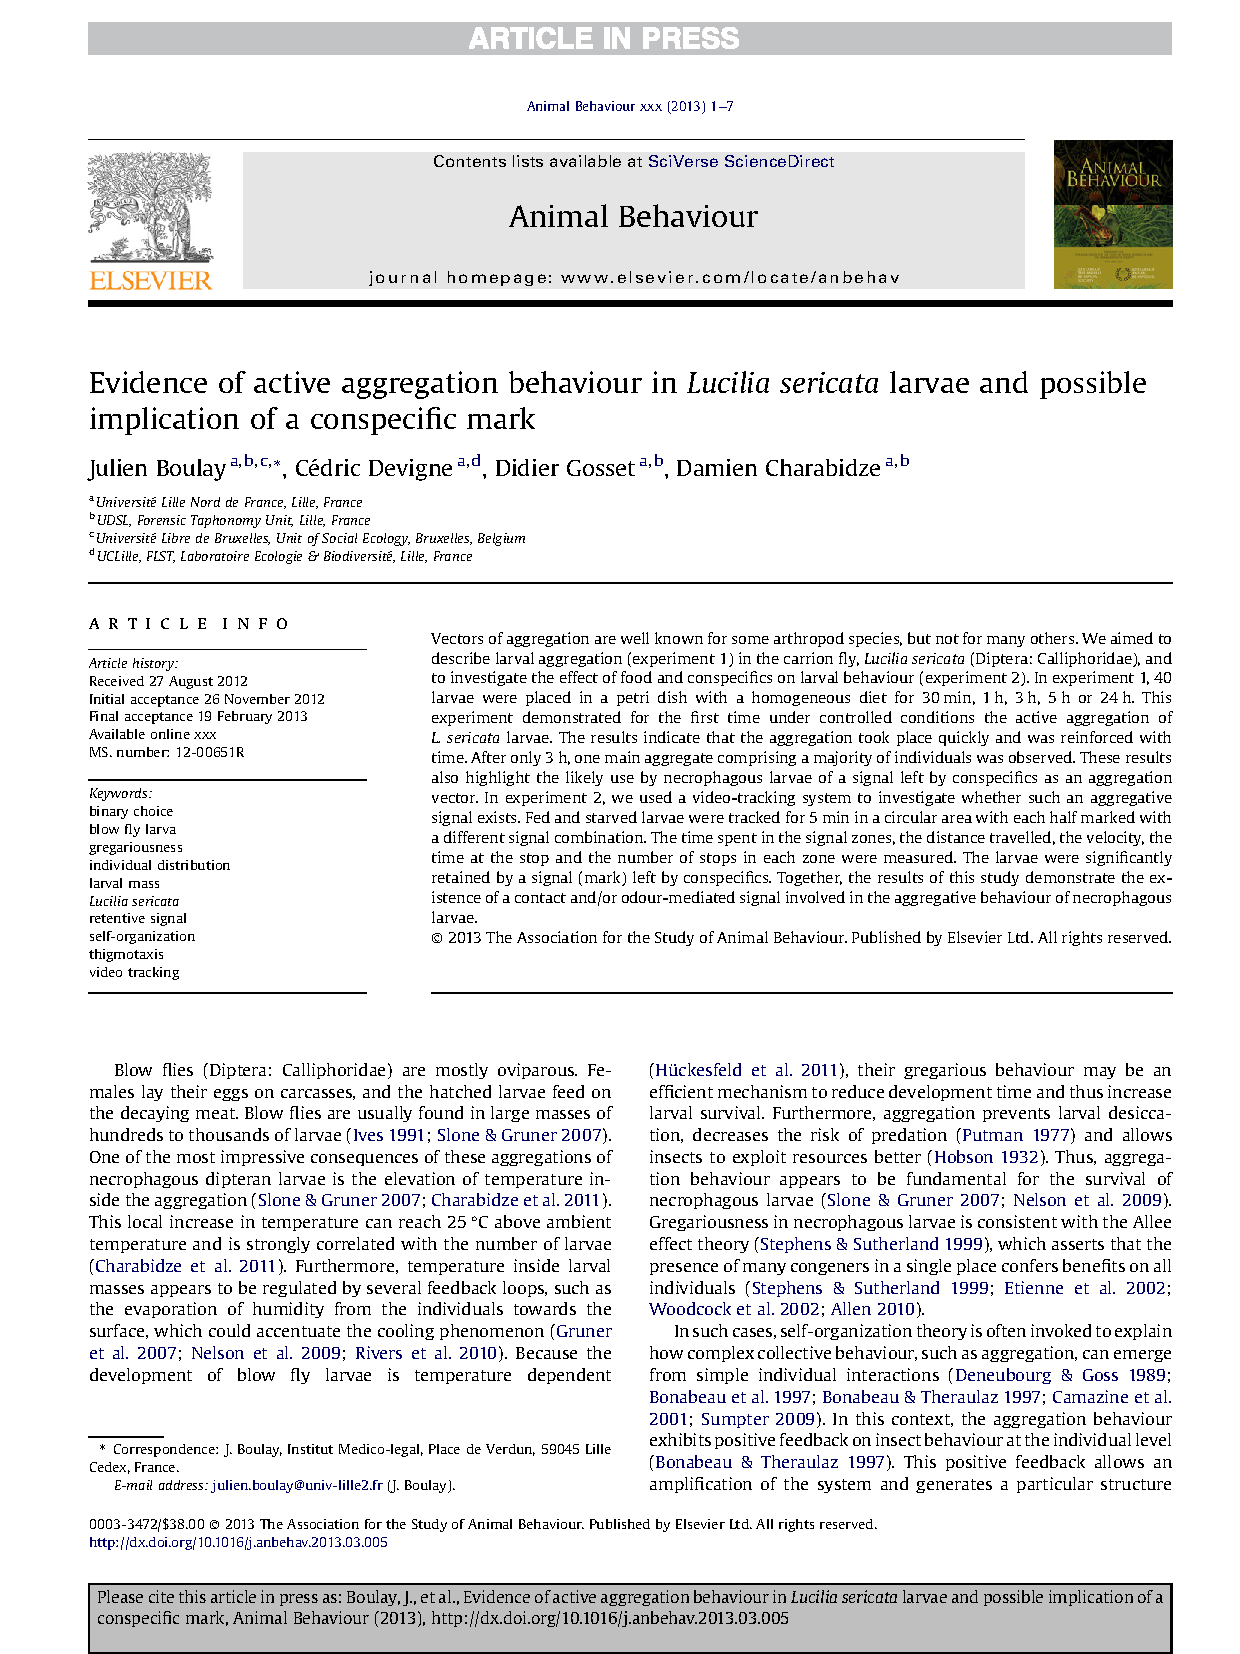
\includepdf[pages=1-7]{ANBEHAV_2013.pdf}
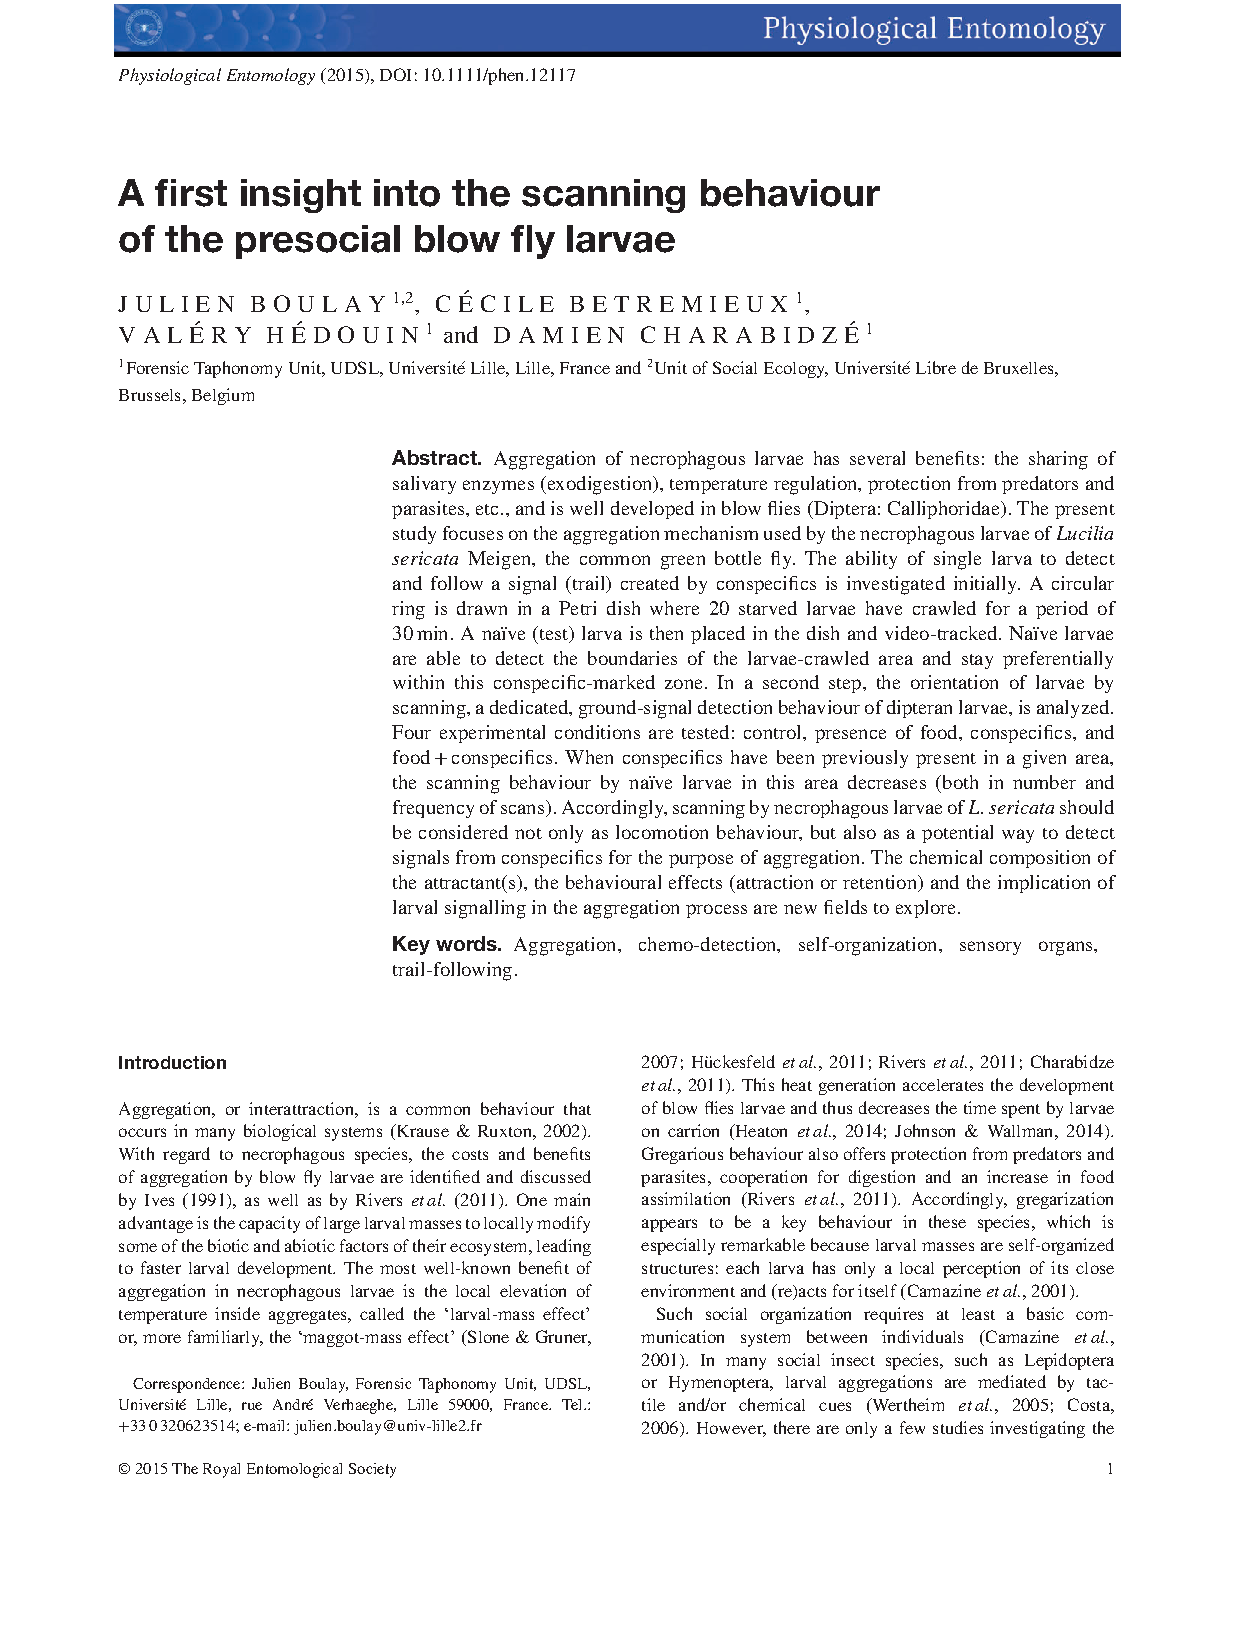
\includepdf[pages=1-8]{PHYENT_2015.pdf}
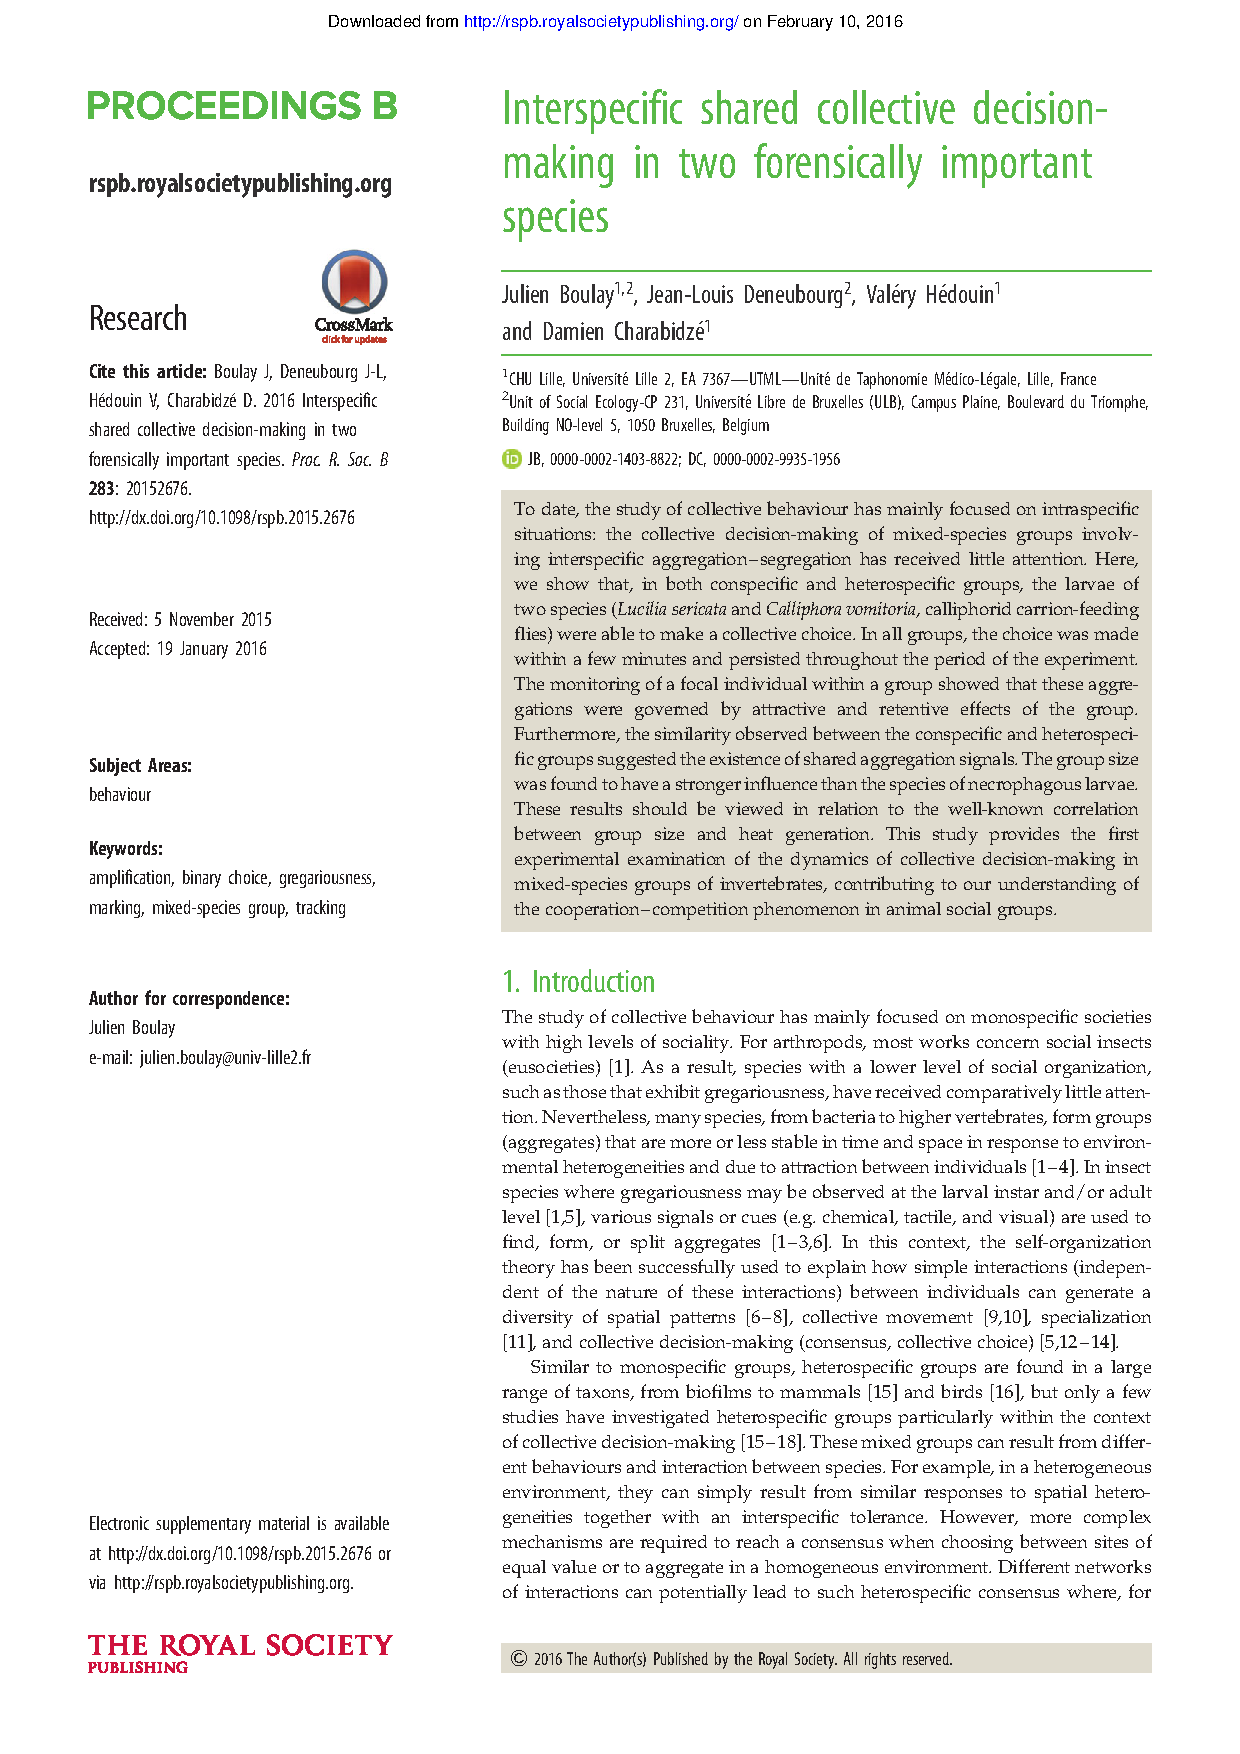
\includepdf[pages=1-9]{PRSB_2016.pdf}
%----------------------------------------------------------------------------------------
%	ANNEXES
%----------------------------------------------------------------------------------------

\chapterimage{blank}
\chapter{Rapports de pré-soutenance}
\includepdf[pages=1-6]{PRE_RAPPORTS_THESE.pdf}

\chapterimage{blank}
\chapter{Rapport de soutenance}

Thèse soutenue à Lille le 16 décembre 2015 devant la commission d'examen composée de :
\begin{itemize} 
\item[\tiny{$\blacksquare$}] \textit{Rapporteurs} \\
\textbf{Jacques \textsc{Gautrais}}\\ Centre de Recherche sur la Cognition Animale (CNRS - Toulouse)\\
\textbf{François \textsc{Verheggen}}\\ Entomologie fonctionnelle et évolutive (Agro-Bio-Tech - Gembloux, Belgique)\\
\end{itemize}

\begin{itemize} 
\item[\tiny{$\blacksquare$}] \textit{Membres} \\
\textbf{Denis \textsc{Fournier}}\\ Unit of Evolutionary biology and Ecology (Université Libre de Bruxelles - Bruxelles, Belgique)\\
\textbf{Prof. Thierry \textsc{Hance}}\\ Écologie des interactions et contrôle biologique (Université Catholique de Louvain - Louvain-la-Neuve, Belgique)\\
\textbf{Prof. Norbert \textsc{Telmon}}\\ UMR 5288 - Laboratoire Anthropologie Moléculaire et Imagerie de Synthèse (CNRS - Toulouse - Section CNU 48 et sous-section 4603)\\
\end{itemize}

\begin{itemize} 
\item[\tiny{$\blacksquare$}] \textit{Directeurs} \\
\textbf{Prof. Valéry \textsc{Hédouin}}\\ Unité de Taphonomie Médico-légale (EA 7367) (Université de Lille - Section CNU 48 et sous-section 4603)\\
\textbf{Prof. Jean-Louis \textsc{Deneubourg}}\\ Unité d'Écologie Sociale (Université Libre de Bruxelles - Bruxelles, Belgique)\\
\end{itemize}

\begin{itemize} 
\item[\tiny{$\blacksquare$}] \textit{Co-Directeur} \\
\textbf{Damien \textsc{Charabidzé}}\\ Unité de Taphonomie Médico-légale (EA 7367) (Université de Lille - Sections CNU 67 et 68)
\end{itemize}

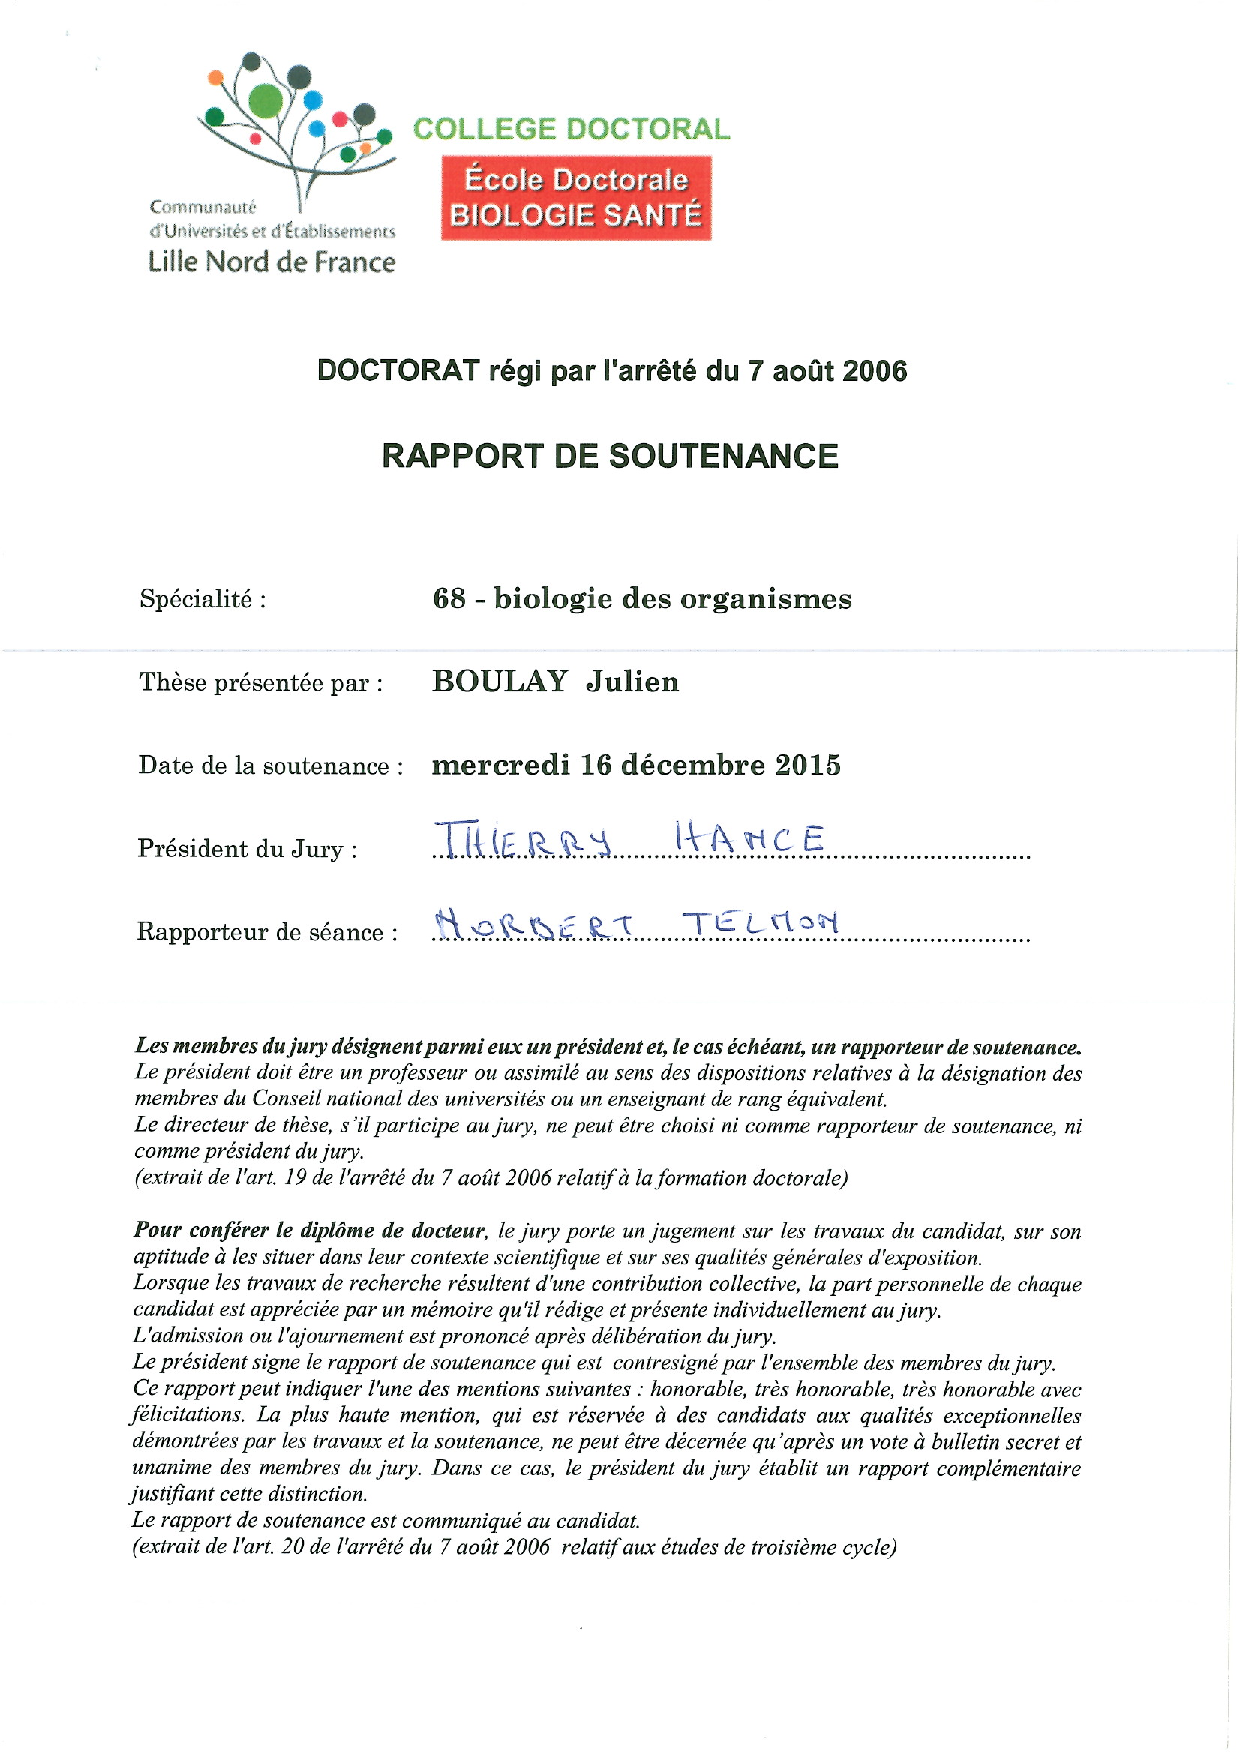
\includepdf[pages=1-6]{RAPPORT_SOUT_THESE.pdf}

\chapterimage{blank}
\chapter{Diplômes de Doctorat}
\includepdf{DiplomeDoctoratULB_BoulayJulien.pdf}
\includepdf{DiplomeDoctoratUnivLILLE_BoulayJulien.pdf}

\chapterimage{blank}
\chapter{Diplôme de Master}
\includepdf[pages=2]{Attestation_Master.pdf}

\chapterimage{blank}
\chapter{Diplôme de Licence}
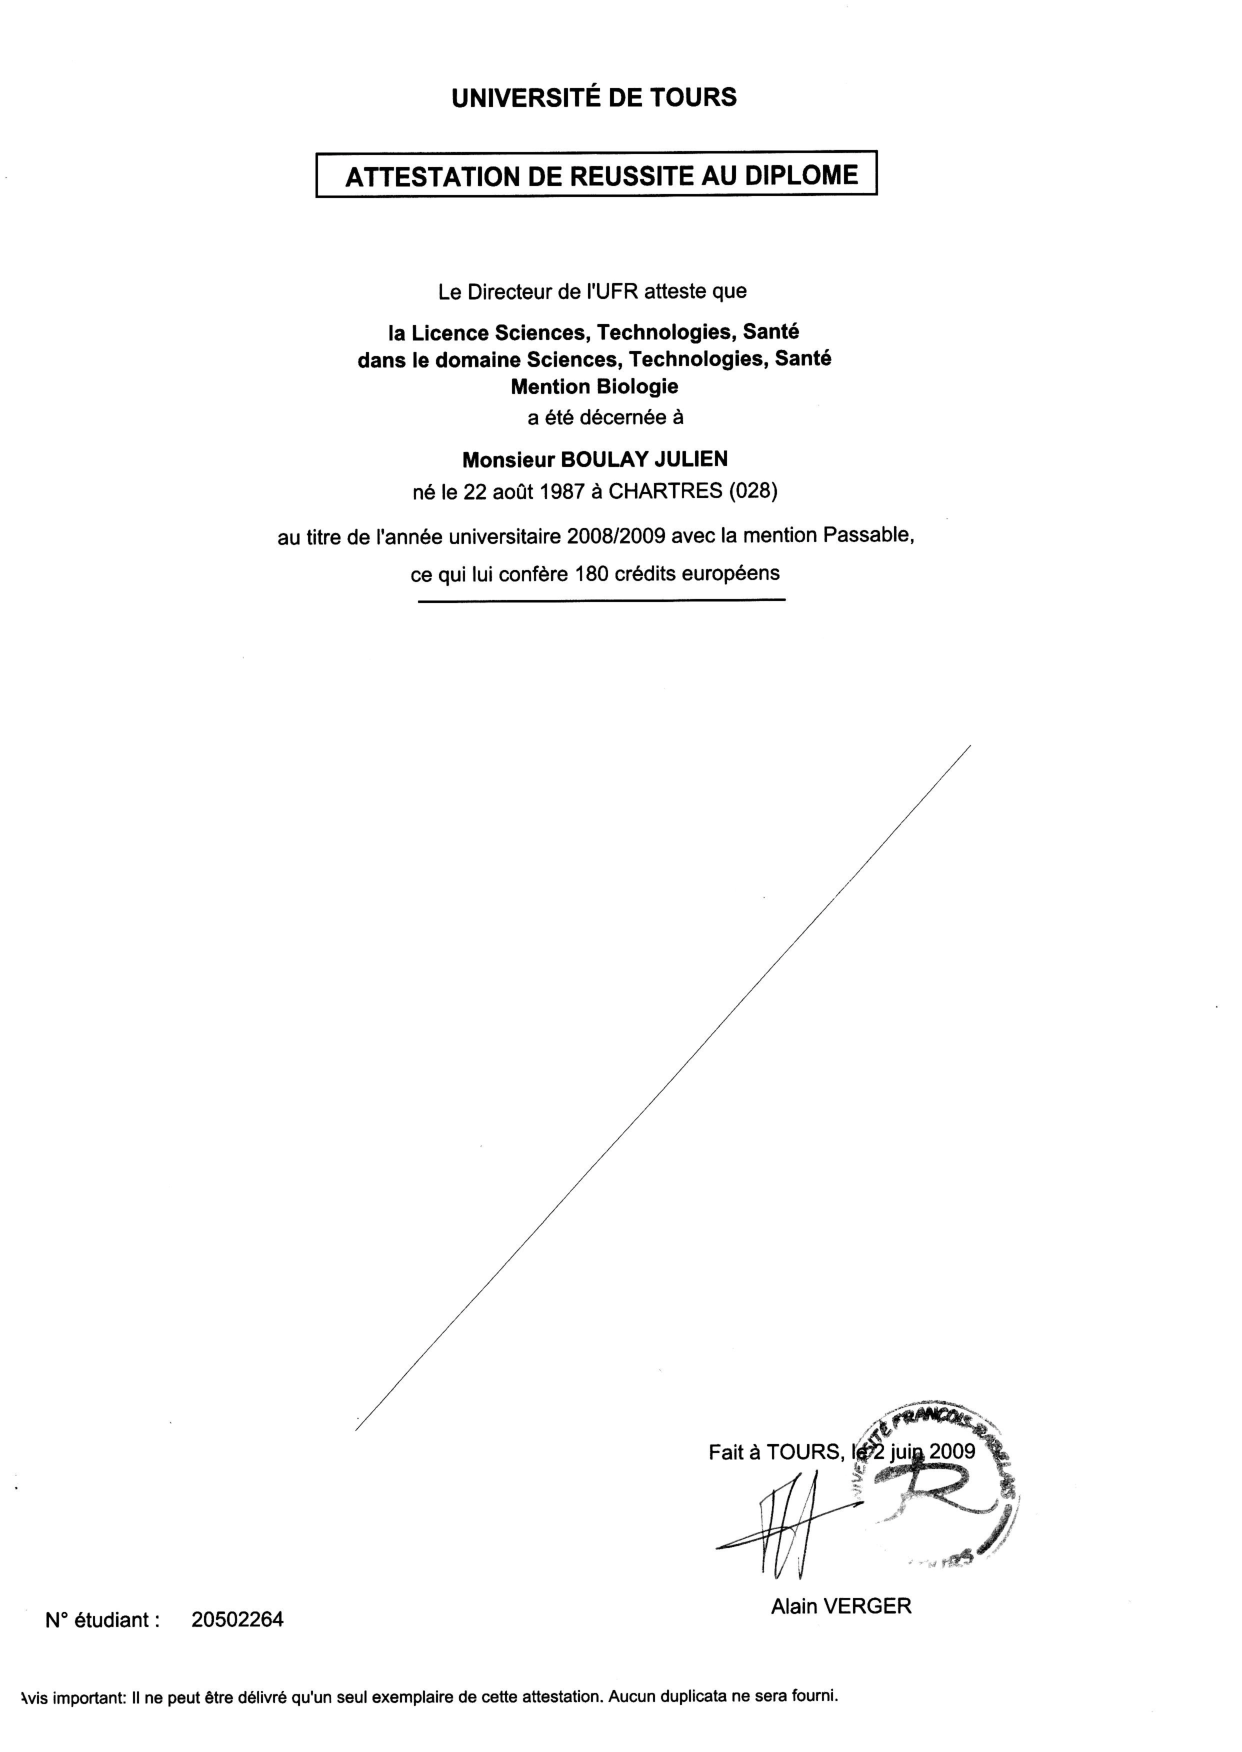
\includepdf{Attestation_Licence.pdf}

\chapterimage{blank}
\chapter{Attestation de recherche}
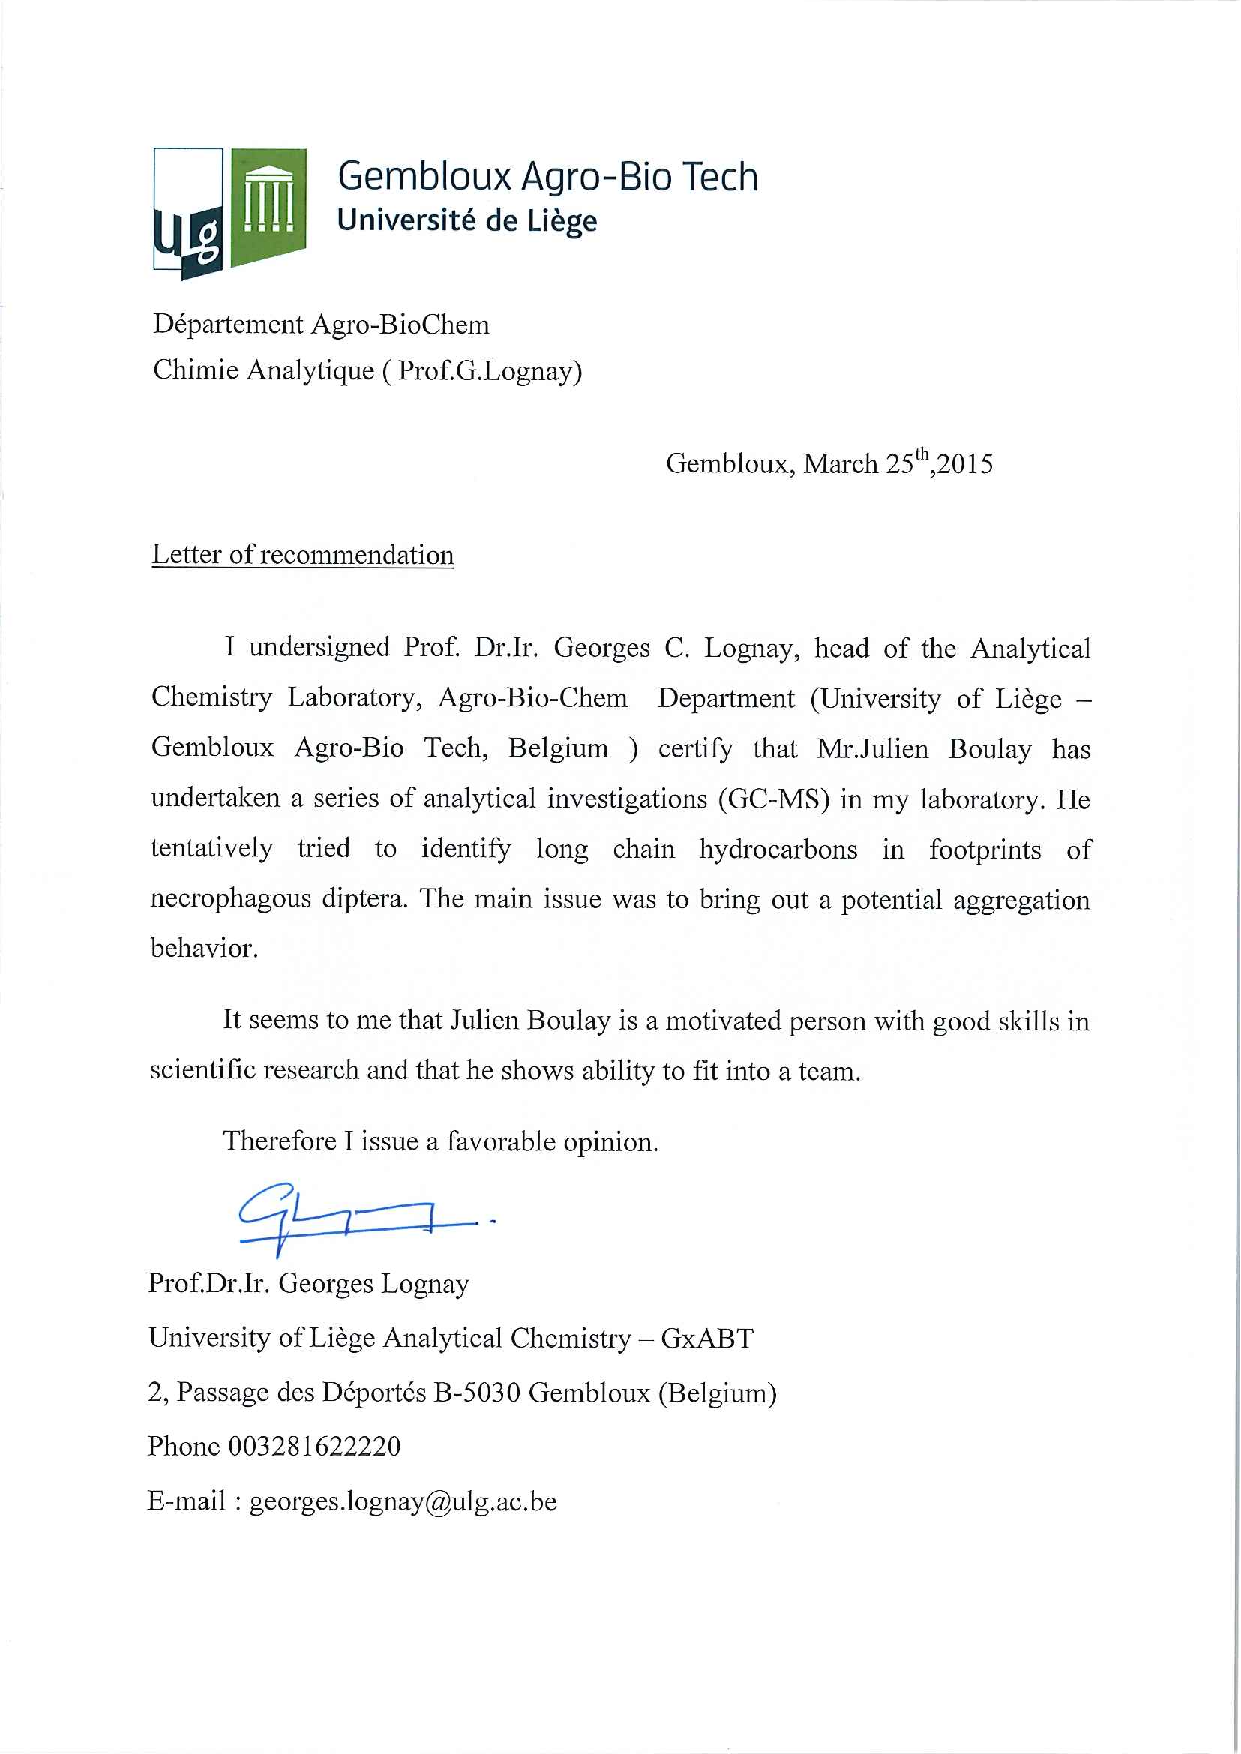
\includepdf{lettre_GeorgesLognay.pdf}

\chapterimage{blank}
\chapter{Attestation d'encadrements}
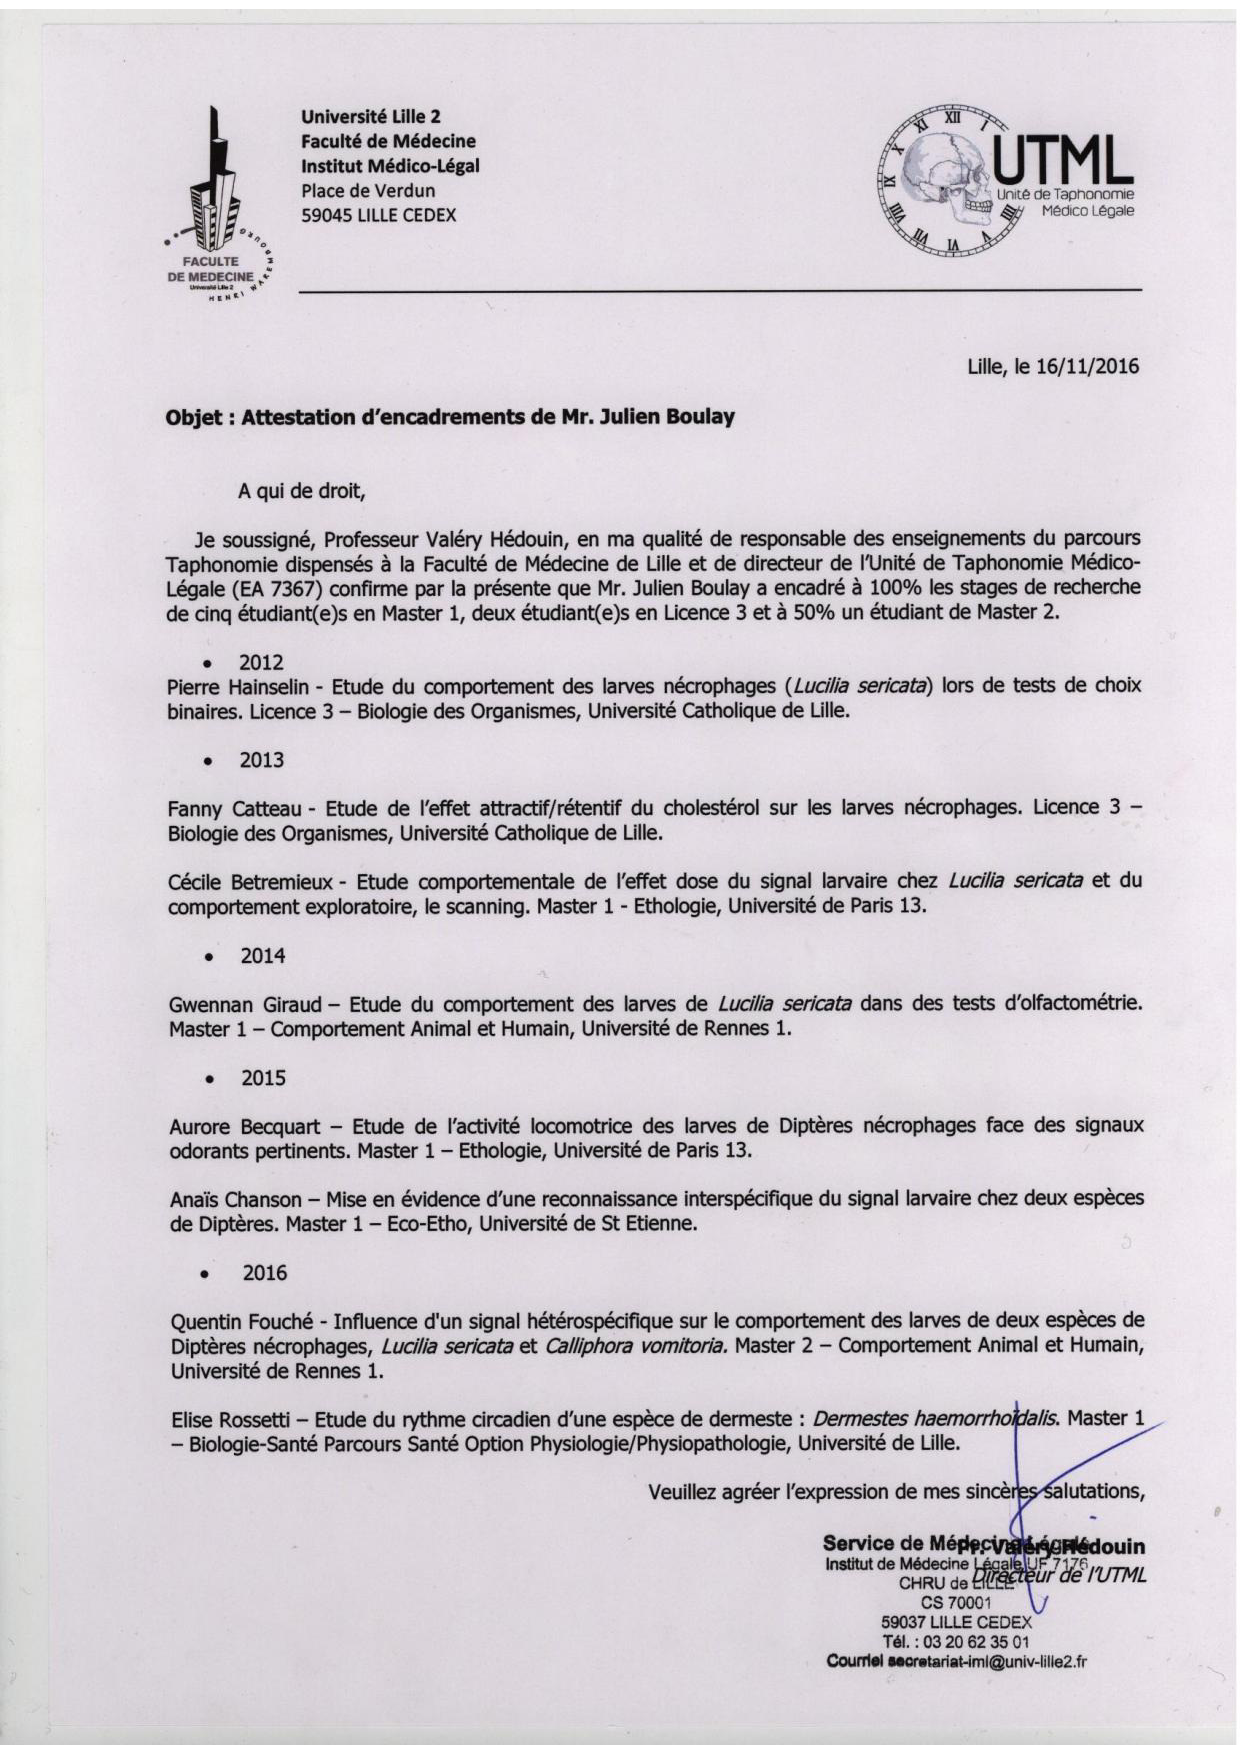
\includepdf{attestation_encadrements_VH.pdf}

\chapterimage{blank}
\chapter{Attestations d'enseignements}
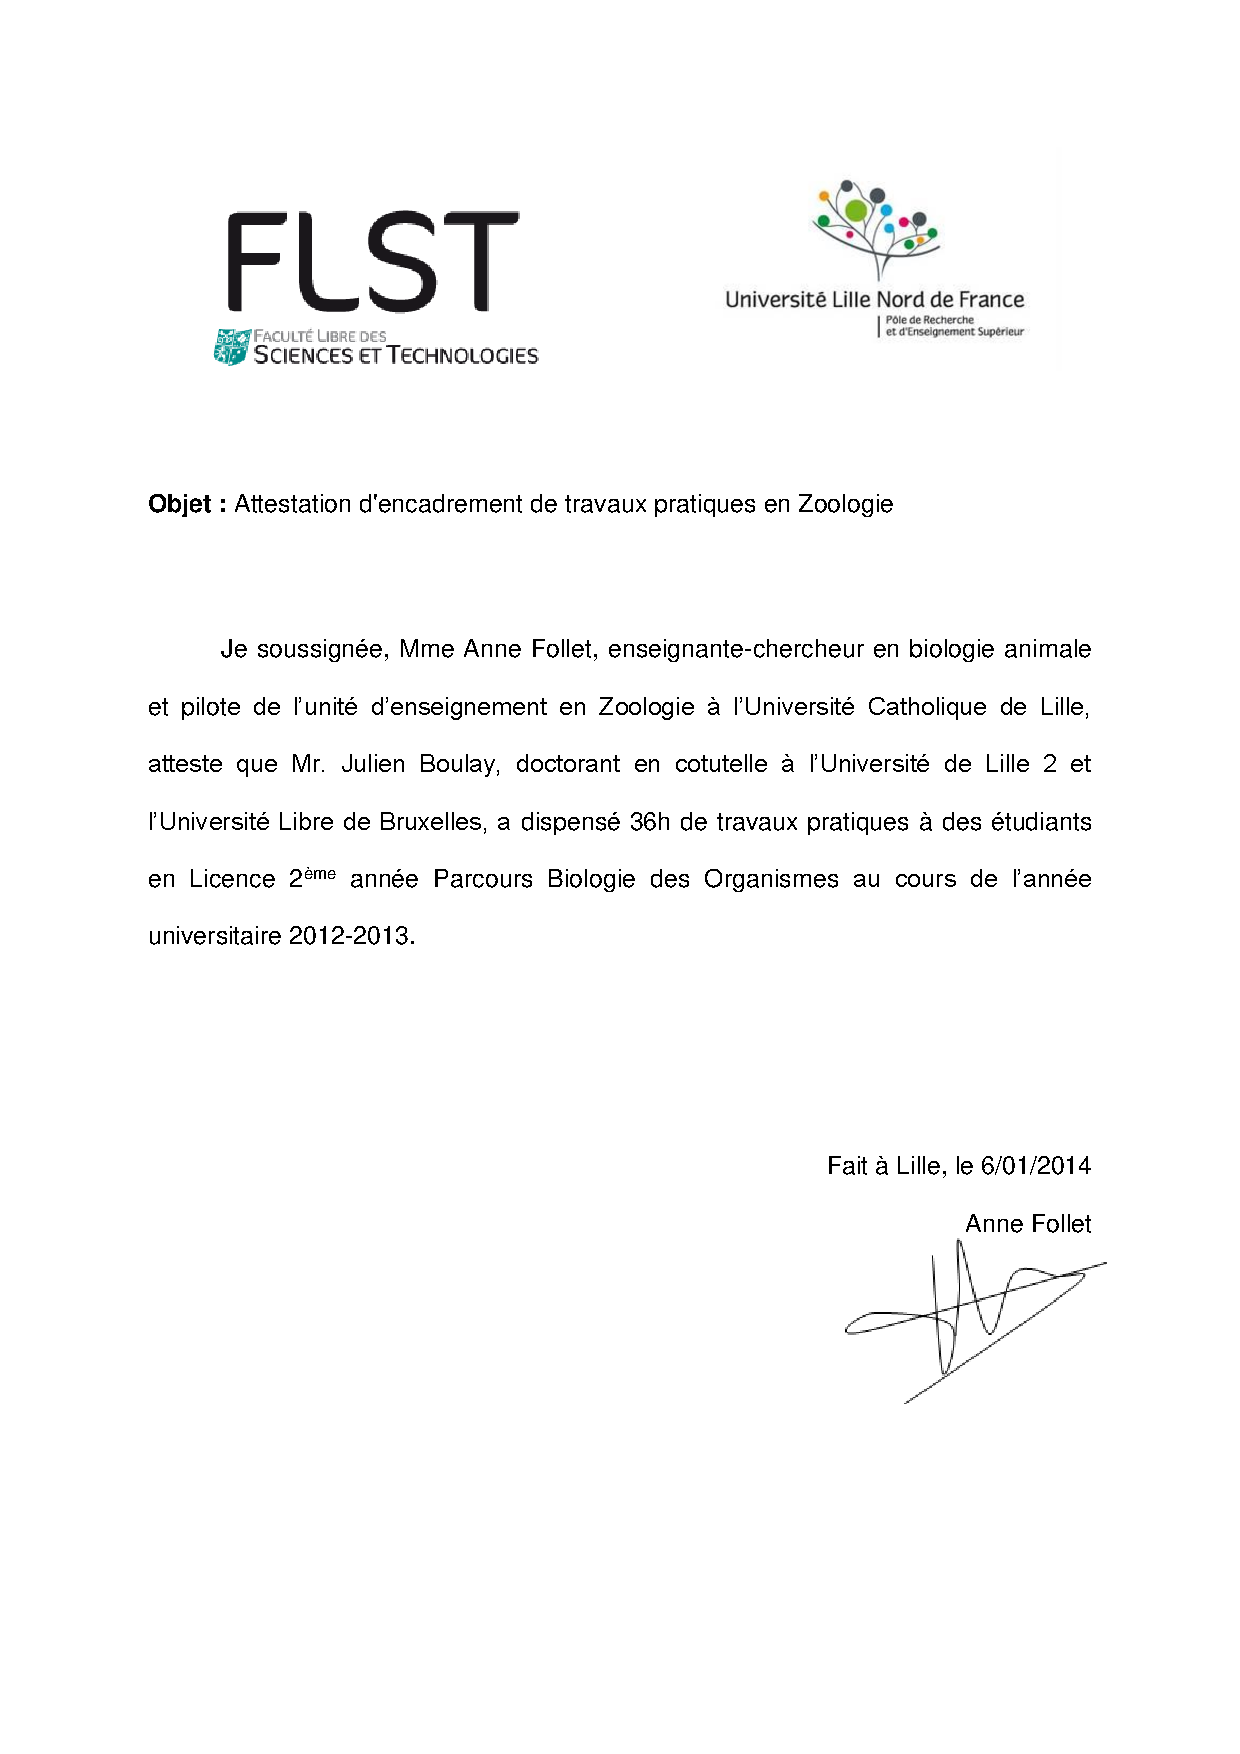
\includepdf{attestation_TP_Zoologie.pdf}
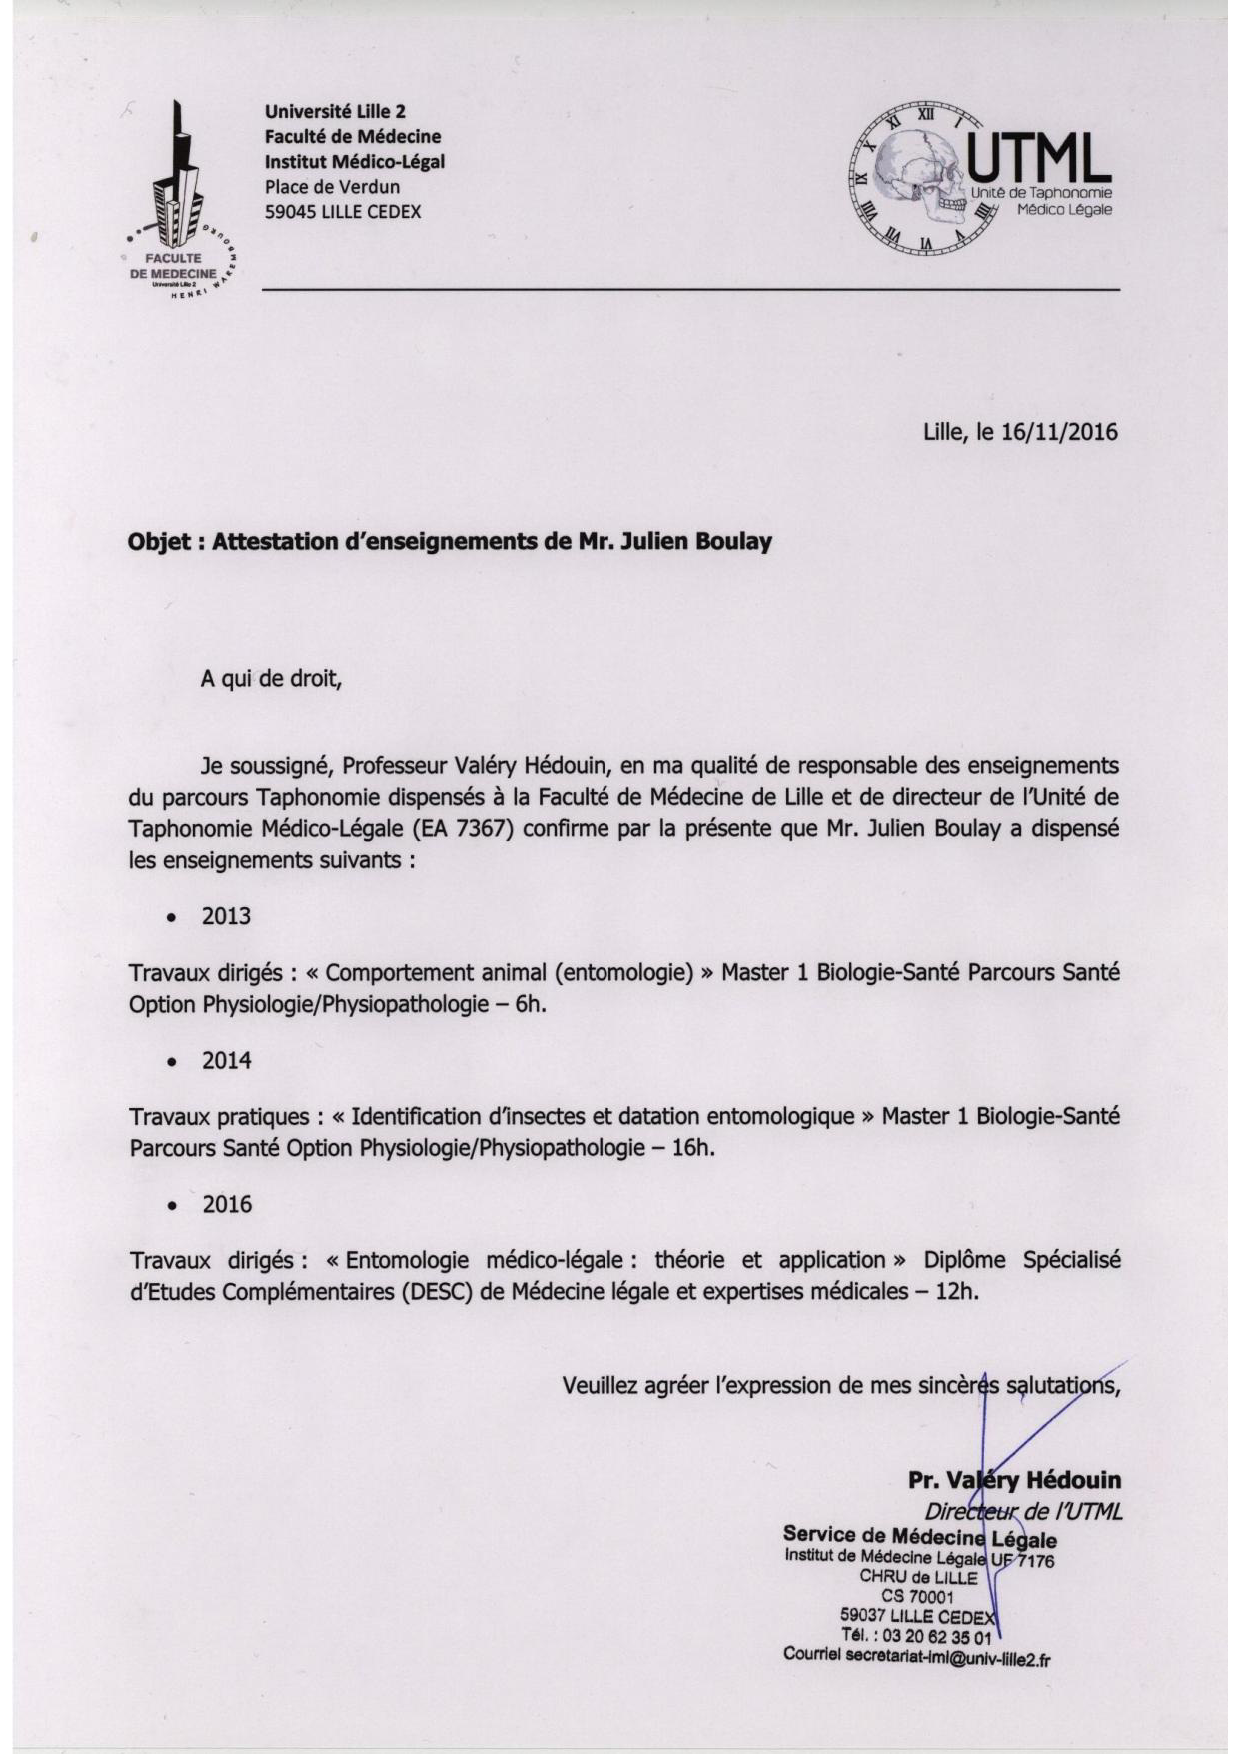
\includepdf{attestation_enseignements_VH.pdf}

\chapterimage{blank}
\chapter{Attestations de responsabilités collectives}
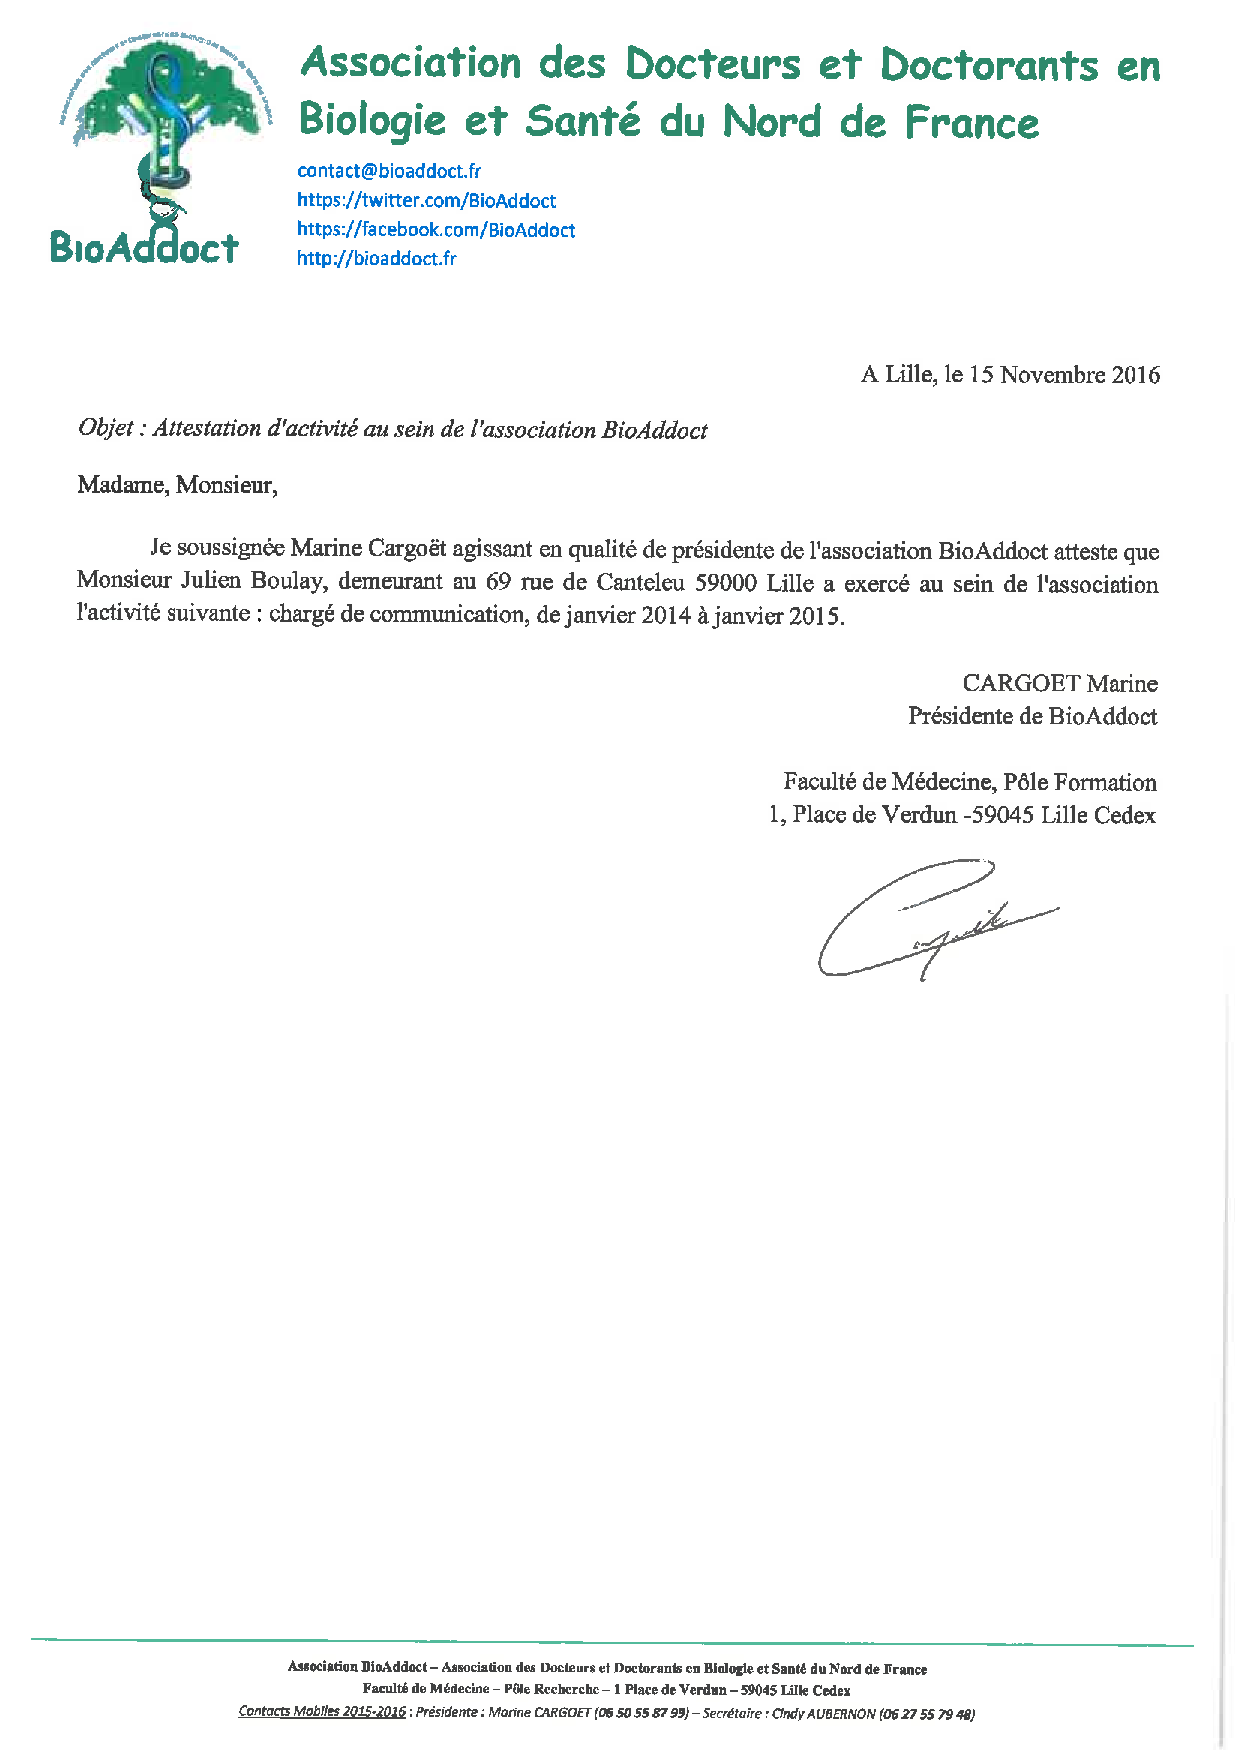
\includepdf{Attestation_bioaddoct.pdf}
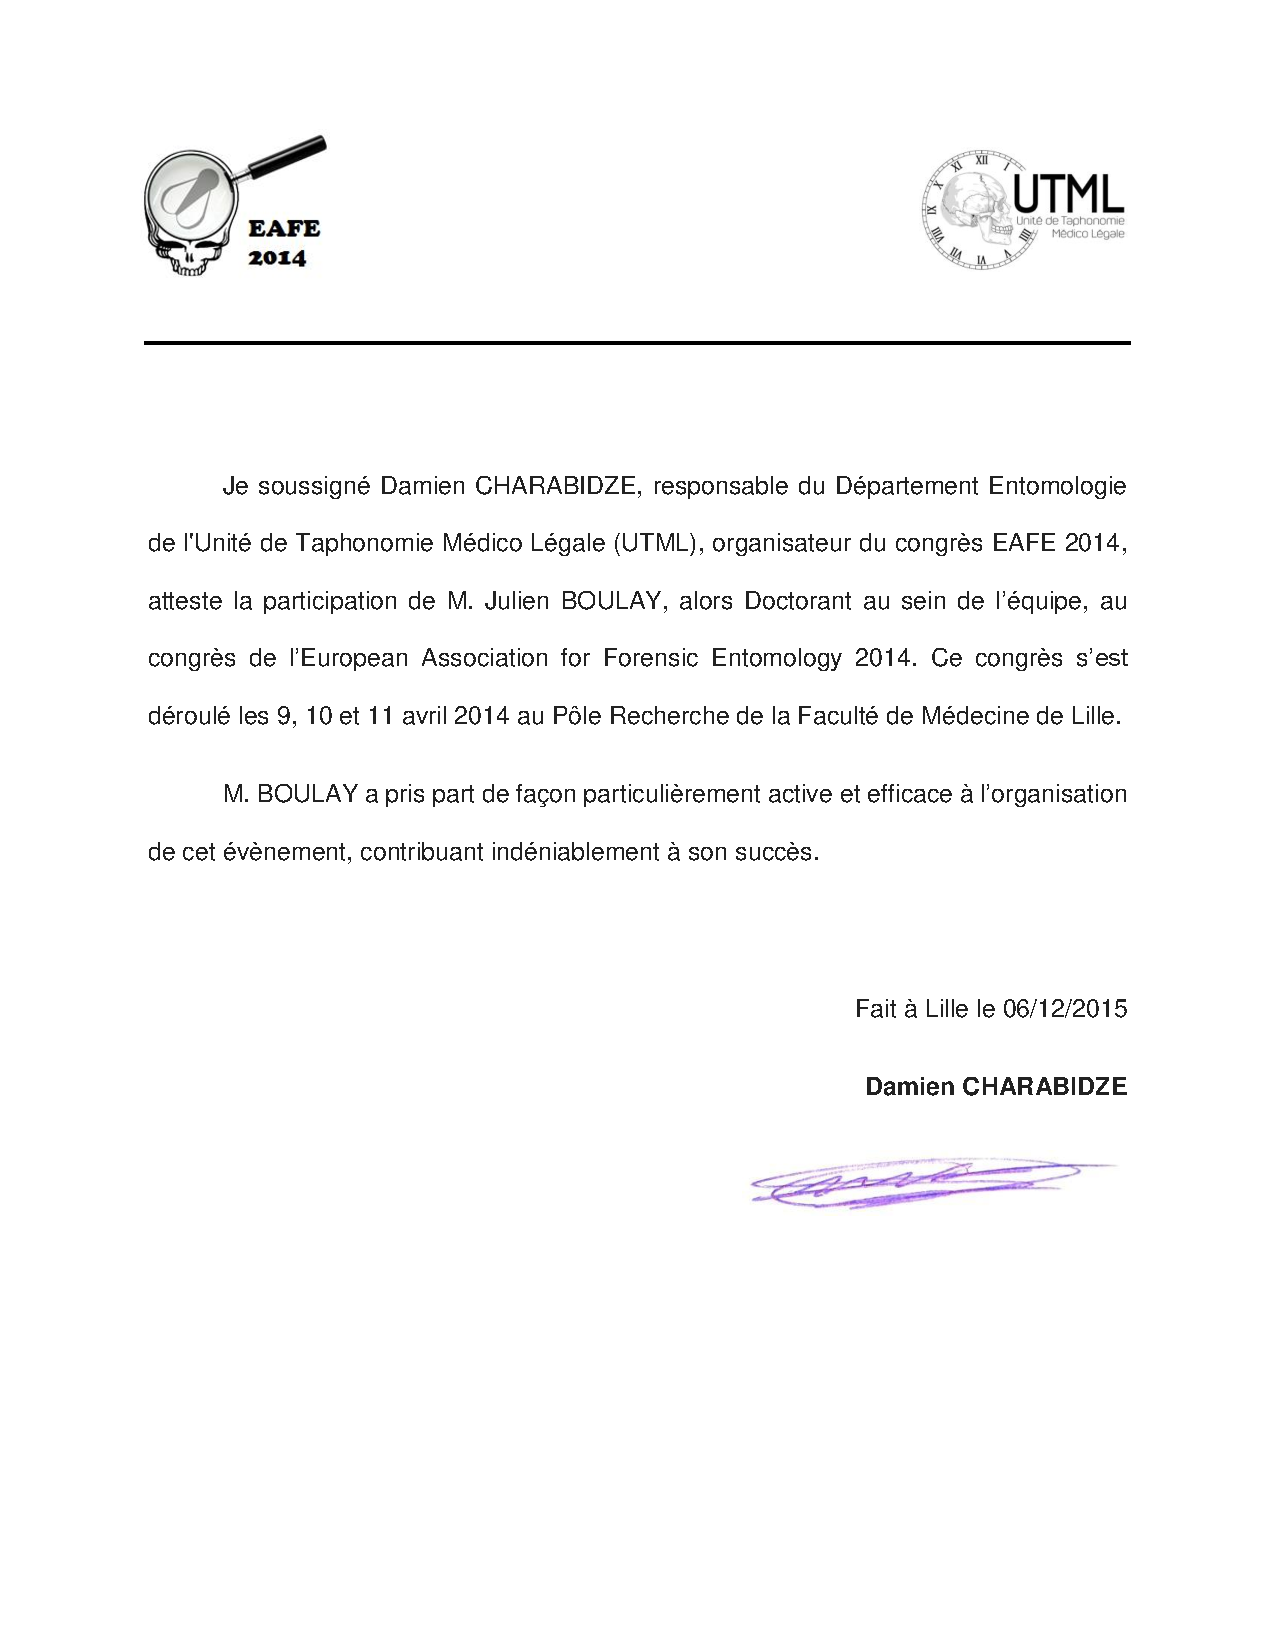
\includepdf{participation_eafe2014.pdf}

\end{document}